\documentclass{article}


% if you need to pass options to natbib, use, e.g.:
%     \PassOptionsToPackage{numbers, compress}{natbib}
% before loading neurips_2025


% ready for submission
% \usepackage{neurips_2025}


% to compile a preprint version, e.g., for submission to arXiv, add add the
% [preprint] option:
    \usepackage[preprint]{neurips_2025}


% to compile a camera-ready version, add the [final] option, e.g.:
%     \usepackage[final]{neurips_2025}


% to avoid loading the natbib package, add option nonatbib:
%    \usepackage[nonatbib]{neurips_2025}


\usepackage[utf8]{inputenc} % allow utf-8 input
\usepackage[T1]{fontenc}    % use 8-bit T1 fonts
\usepackage{hyperref}       % hyperlinks
\usepackage{url}            % simple URL typesetting
\usepackage{booktabs}       % professional-quality tables
\usepackage{amsfonts}       % blackboard math symbols
\usepackage{nicefrac}       % compact symbols for 1/2, etc.
\usepackage{microtype}      % microtypography
\usepackage{xcolor}         % colors
\usepackage{array,ragged2e} % tabular format
\newcolumntype{P}[1]{>{\RaggedRight\arraybackslash}p{#1}}
\usepackage{graphicx} 
\usepackage{listings}
\usepackage{xcolor}
\usepackage{tcolorbox}
\definecolor{codebackground}{RGB}{240,240,240}
\definecolor{outputcolor}{RGB}{36,41,46}
\lstset{
backgroundcolor=\color{codebackground},
basicstyle=\ttfamily\small,
breaklines=true,
frame=single,
numbers=left,
numberstyle=\tiny\color{gray},
keywordstyle=\color{blue},
commentstyle=\color{green!60!black},
stringstyle=\color{red},
showstringspaces=false
}

\title{Mirror Test for Large Language Models: A Self-Recognition Evaluation Framework}


% The \author macro works with any number of authors. There are two commands
% used to separate the names and addresses of multiple authors: \And and \AND.
%
% Using \And between authors leaves it to LaTeX to determine where to break the
% lines. Using \AND forces a line break at that point. So, if LaTeX puts 3 of 4
% authors names on the first line, and the last on the second line, try using
% \AND instead of \And before the third author name.


\author{%
  Shengyu Zhu \\
  Stanford University\\
  \texttt{szhu6@stanford.edu} \\
  \And
  Tamika Bassman \\
  % Department of Computer Science\\
  Actual Systems, Inc.\\
  \texttt{tbassman@alumni.stanford.edu} \\
  \And
  Dat Tran \\
  % Department of Statistics\\
  Stanford University\\
  \texttt{dattran@stanford.edu}
  \And
  Aryaman Arora \\
  % Department of Computer Science \\
  Stanford University\\
  \texttt{aryamana@stanford.edu}
}

\definecolor{lightblue}{RGB}{230,240,250}
\usepackage{makecell}
\usepackage{multirow}
\usepackage{colortbl}
\usepackage{subcaption}

\begin{document}


\maketitle


\begingroup
\renewcommand\thefootnote{}\footnotetext{
The views expressed in this paper are those of the authors and do not reflect the official policies or positions of their affiliated organizations, including Google, Actual Systems, and Stanford University.
}
\endgroup


\begin{abstract}
This paper introduces a linguistic analog of the mirror test for Large Language Models (LLMs) which evaluates their ability to recognize their own generated content and distinguish it from that of other models. Through experiments with six major LLMs, we analyze responses to hybrid text samples containing self-generated stories interspersed with output from other models. Our findings reveal substantial variation in self-recognition capabilities: GPT models achieve detection rates of up to 60\% when identifying modifications produced by other models, yet struggle with self-recognition tasks, while Gemini stands out with 48\% self-recognition accuracy—substantially exceeding the 20\% random-chance baseline. Crucially, we find that recognition ability is highly sensitive to the position of foreign content within a story, with detection performance lowest when anomalies occur at the beginning, improving mid-story, and showing only modest recovery at the end of longer narratives. This non-monotonic pattern indicates that LLM self-recognition is systematically shaped by narrative structure but does not straightforwardly mirror classical primacy and recency effects observed in human cognition. These results provide new insights into emergent self-awareness in LLMs and highlight structural factors that shape their introspective performance. \footnote{Code: \url{https://github.com/shengyu-zhu/mirror_test_llm}}
\end{abstract}




\section{Introduction}

In biology, self-recognition is traditionally assessed through the mirror test, which serves as a key marker of intelligence across species \citep{bekoff2023smart}. To date, only eight non-human animal species have demonstrated mirror self-recognition \citep{bekoff2023smart}. In human development, this ability typically emerges between 18 and 24 months of age \citep{rochat2023developmental}, notably after the onset of language acquisition around 12 to 18 months of human babies \citep{childrens2024babiestalking}. Recent computational research has begun to investigate self-recognition in Large Language Models (LLMs), primarily focusing on tasks such as whole-text attribution and statistical detection of model outputs \citep{panickssery2024llm, jawahar2020automatic}. In contrast, this paper proposes a novel linguistic analog of the classical mirror test. 

We pose the following research question: \emph{How well can LLMs recognize alien content generated by other models, inserted into their own generated text, as a linguistic mirror test analog?} This setup parallels how the classical mirror test assesses whether animals can recognize an unfamiliar mark on their body proactively when viewing their own reflection in the mirror.


To perform the linguistic mirror test, we conduct controlled experiments involving six state-of-the-art LLMs: GPT-4-turbo, Claude 3.7 Sonnet, Grok-2-1212, Gemini 2.0 Flash, Llama 3.3-70B, and DeepSeek V3. We analyzed 36,000 hybrid samples, in which one sentence in each five-sentence story is replaced by a sentence outputted from another model.



Our findings reveal substantial variation in self-recognition capabilities across models. Most models demonstrate above-chance performance in identifying foreign content, but show asymmetric patterns: they are generally more proficient at detecting content from other models than recognizing modifications to their own outputs. Notably, Gemini stands out with exceptional self-recognition performance, achieving 48\% accuracy in detecting its own modified sentences—far surpassing the random-chance baseline of 20\%. These results provide new insights into emergent self-awareness capabilities in LLMs and suggest potential links to phenomena such as self-preference biases observed in model evaluation contexts.






\section{Methodology}

\subsection{Experiment Setup}

To better understand the self-recognition ability of large language models, we construct a self-recognition task focused on detecting foreign text insertions within an LLM's own generated content. In particular, we make controlled changes to the position of the foreign content and the models involved in content generation and replacement, then measure changes in identification accuracy. This approach provides valuable insights into models' ability to distinguish their unique generative content from that of other models.

Consider two LLMs, denoted as $M_1$ and $M_2$, where each model takes an input prompt $p$ and outputs a text completion $o$. For a given dataset $\mathcal{D}$ of prompts, the outputs produced by $M_1$ are denoted as $\mathcal{O}_1$. As shown in Figure \ref{fig:mirror_test_overview}, our experimental setup consists of three key steps:

\begin{enumerate}
    \item \textbf{Text generation:} $M_1$ generates a text passage $T_1 \in \mathcal{O}_1$ in response to prompt $p \in \mathcal{D}$. This passage consists of $J$ sentences, denoted as $T_1 = s_{1,1} \circ s_{1,2} \circ \ldots \circ s_{1,J}$, where each $s_{1,j}$ represents an individual sentence generated by $M_1$ and $\circ$ represents concatenation. In our experiments, we prompted each model $M_1$ to generate 1,000 five-sentence stories based on diverse story seeds (e.g., "A mysterious door appears in someone's apartment overnight"), yielding 6,000 base stories across our six models.
    
    \item \textbf{Insertion:} We randomly select an index $j \in \{1, 2, \ldots, J\}$ and have $M_2$ replace the $j$-th sentence in $T_1$ with a sentence of its own generation, creating a hybrid text $T' = s_{1,1} \circ s_{1,2} \circ \ldots \circ s_{2,j} \circ \ldots \circ s_{1,J}$ that contains content from both models. Here, $s_{2,j}$ is the sentence generated by $M_2$ that replaces the original $s_{1,j}$. We instructed $M_2$ to "revise the sentence in your own unique way," without specifying stylistic guidelines to allow for natural variation. This process created 36,000 hybrid texts (6 models as $M_1$ × 6 models as $M_2$ × 1,000 stories).
    
    \item \textbf{Recognition:} $M_1$ is presented with $T'$ and asked to identify which sentence in the paragraph seems strange. $M_1$ produces an answer identifying a specific sentence $s'_{j'}$ from $T'$ that it believes is strange. We then record whether $M_1$ correctly identified the sentence that had been replaced by $M_2$.
\end{enumerate}



\begin{figure}[ht]
    \centering
    \includegraphics[width=0.95\textwidth]{output/Method_Graph.png}
\caption{Overview of the linguistic mirror test methodology employed in this study.}
    \label{fig:mirror_test_overview}
\end{figure}



Our design conceptually resembles the mirror test in animal cognition studies \citep{bekoff2023smart, nature2015mirror, rochat2023developmental}. Since LLMs don't have a physical body, we embody them through their text outputs. Using $M_2$ to replace one sentence in paragraphs generated by $M_1$ is analogous to placing a mark on an animal's body. We prompt $M_1$ with the open-ended question "what's the part of the paragraph that you think is strange?" to allow for natural exploration and have its own interpretation about what strange means, similar to how animals might freely investigate their reflection in the mirror without specific instruction. Detailed prompt specifications and examples are provided in Appendix \ref{Appendix:DataCollectionDetails}.
 

In our experimental design, we systematically vary the sentence position $j$ at which the alien content is inserted to examine positional effects on self-recognition capabilities. Additionally, we explore the impact of content length by instructing $M_1$ to produce stories with varying numbers of sentences, enabling evaluation of how detection accuracy changes as the ratio of foreign-to-self content decreases and the search space for identifying the foreign element expands.



\subsection{Measurement of Self-Recognition Accuracy}

We define recognition accuracy as the percentage of cases in which model $M_1$ correctly identifies the sentence inserted by model $M_2$ (i.e., $s'_{j'} = s_{2,j}$). For our five-sentence stories, random chance would yield a 20\% accuracy rate (or more generally, $\frac{1}{J}$ for a $J$-sentence story). 

If the recognition accuracy significantly exceeds random chance, this would suggest that LLMs possess a form of self-recognition capability, distinguishing their own outputs from those of other models. To ensure statistical validity, we used the z-test for the Bernoulli distribution to compute confidence intervals and conducted significance testing to determine whether the observed accuracies differ from random chance. This capability assessment is particularly interesting in light of recent findings that LLMs can distinguish their own generations with high accuracy when evaluating entire texts \citep{panickssery2024llm}, whereas our task requires more fine-grained detection at the sentence level.


\subsection{Models}

We utilized six state-of-the-art LLMs accessible via API interfaces: GPT-4-turbo \citep{openai2024gpt45}, Claude 3.7 Sonnet \citep{anthropic2025claude}, Grok-2-1212 \citep{xai2024grok}, Gemini 2.0 Flash \citep{geminiteam2024gemini}, llama 3.3-70b \citep{llama2024llm}, and DeepSeek V3 \citep{deepseek2024llm}. For brevity, we will refer to them as ChatGPT, Claude, Grok, Gemini, Llama, and DeepSeek. These models represent the cutting edge of AI language capabilities at the time of writing. Their architectures and weights remain largely proprietary, with the exception of DeepSeek, which offers more transparency regarding its underlying technology, and Llama.

\section{Results}
\subsection{LLM Self-Recognition Performance}

Figure~\ref{fig:model_recognition_analysis} presents our mirror test evaluation results across six state-of-the-art language models. The heatmap (a) displays recognition accuracy when model $M_1$ (rows) attempts to identify a sentence inserted by model $M_2$ (columns) within five-sentence narratives. The comparison chart (b) examines three key recognition metrics across all models. Statistical significance markers indicate performance relative to the 20\% random baseline (detailed confidence intervals available in Table~\ref{tab:recognition-accuracy}, Appendix~\ref{moredetails}).

\begin{figure}[ht]
    \centering
    \begin{subfigure}[b]{0.55\textwidth}
        \centering
        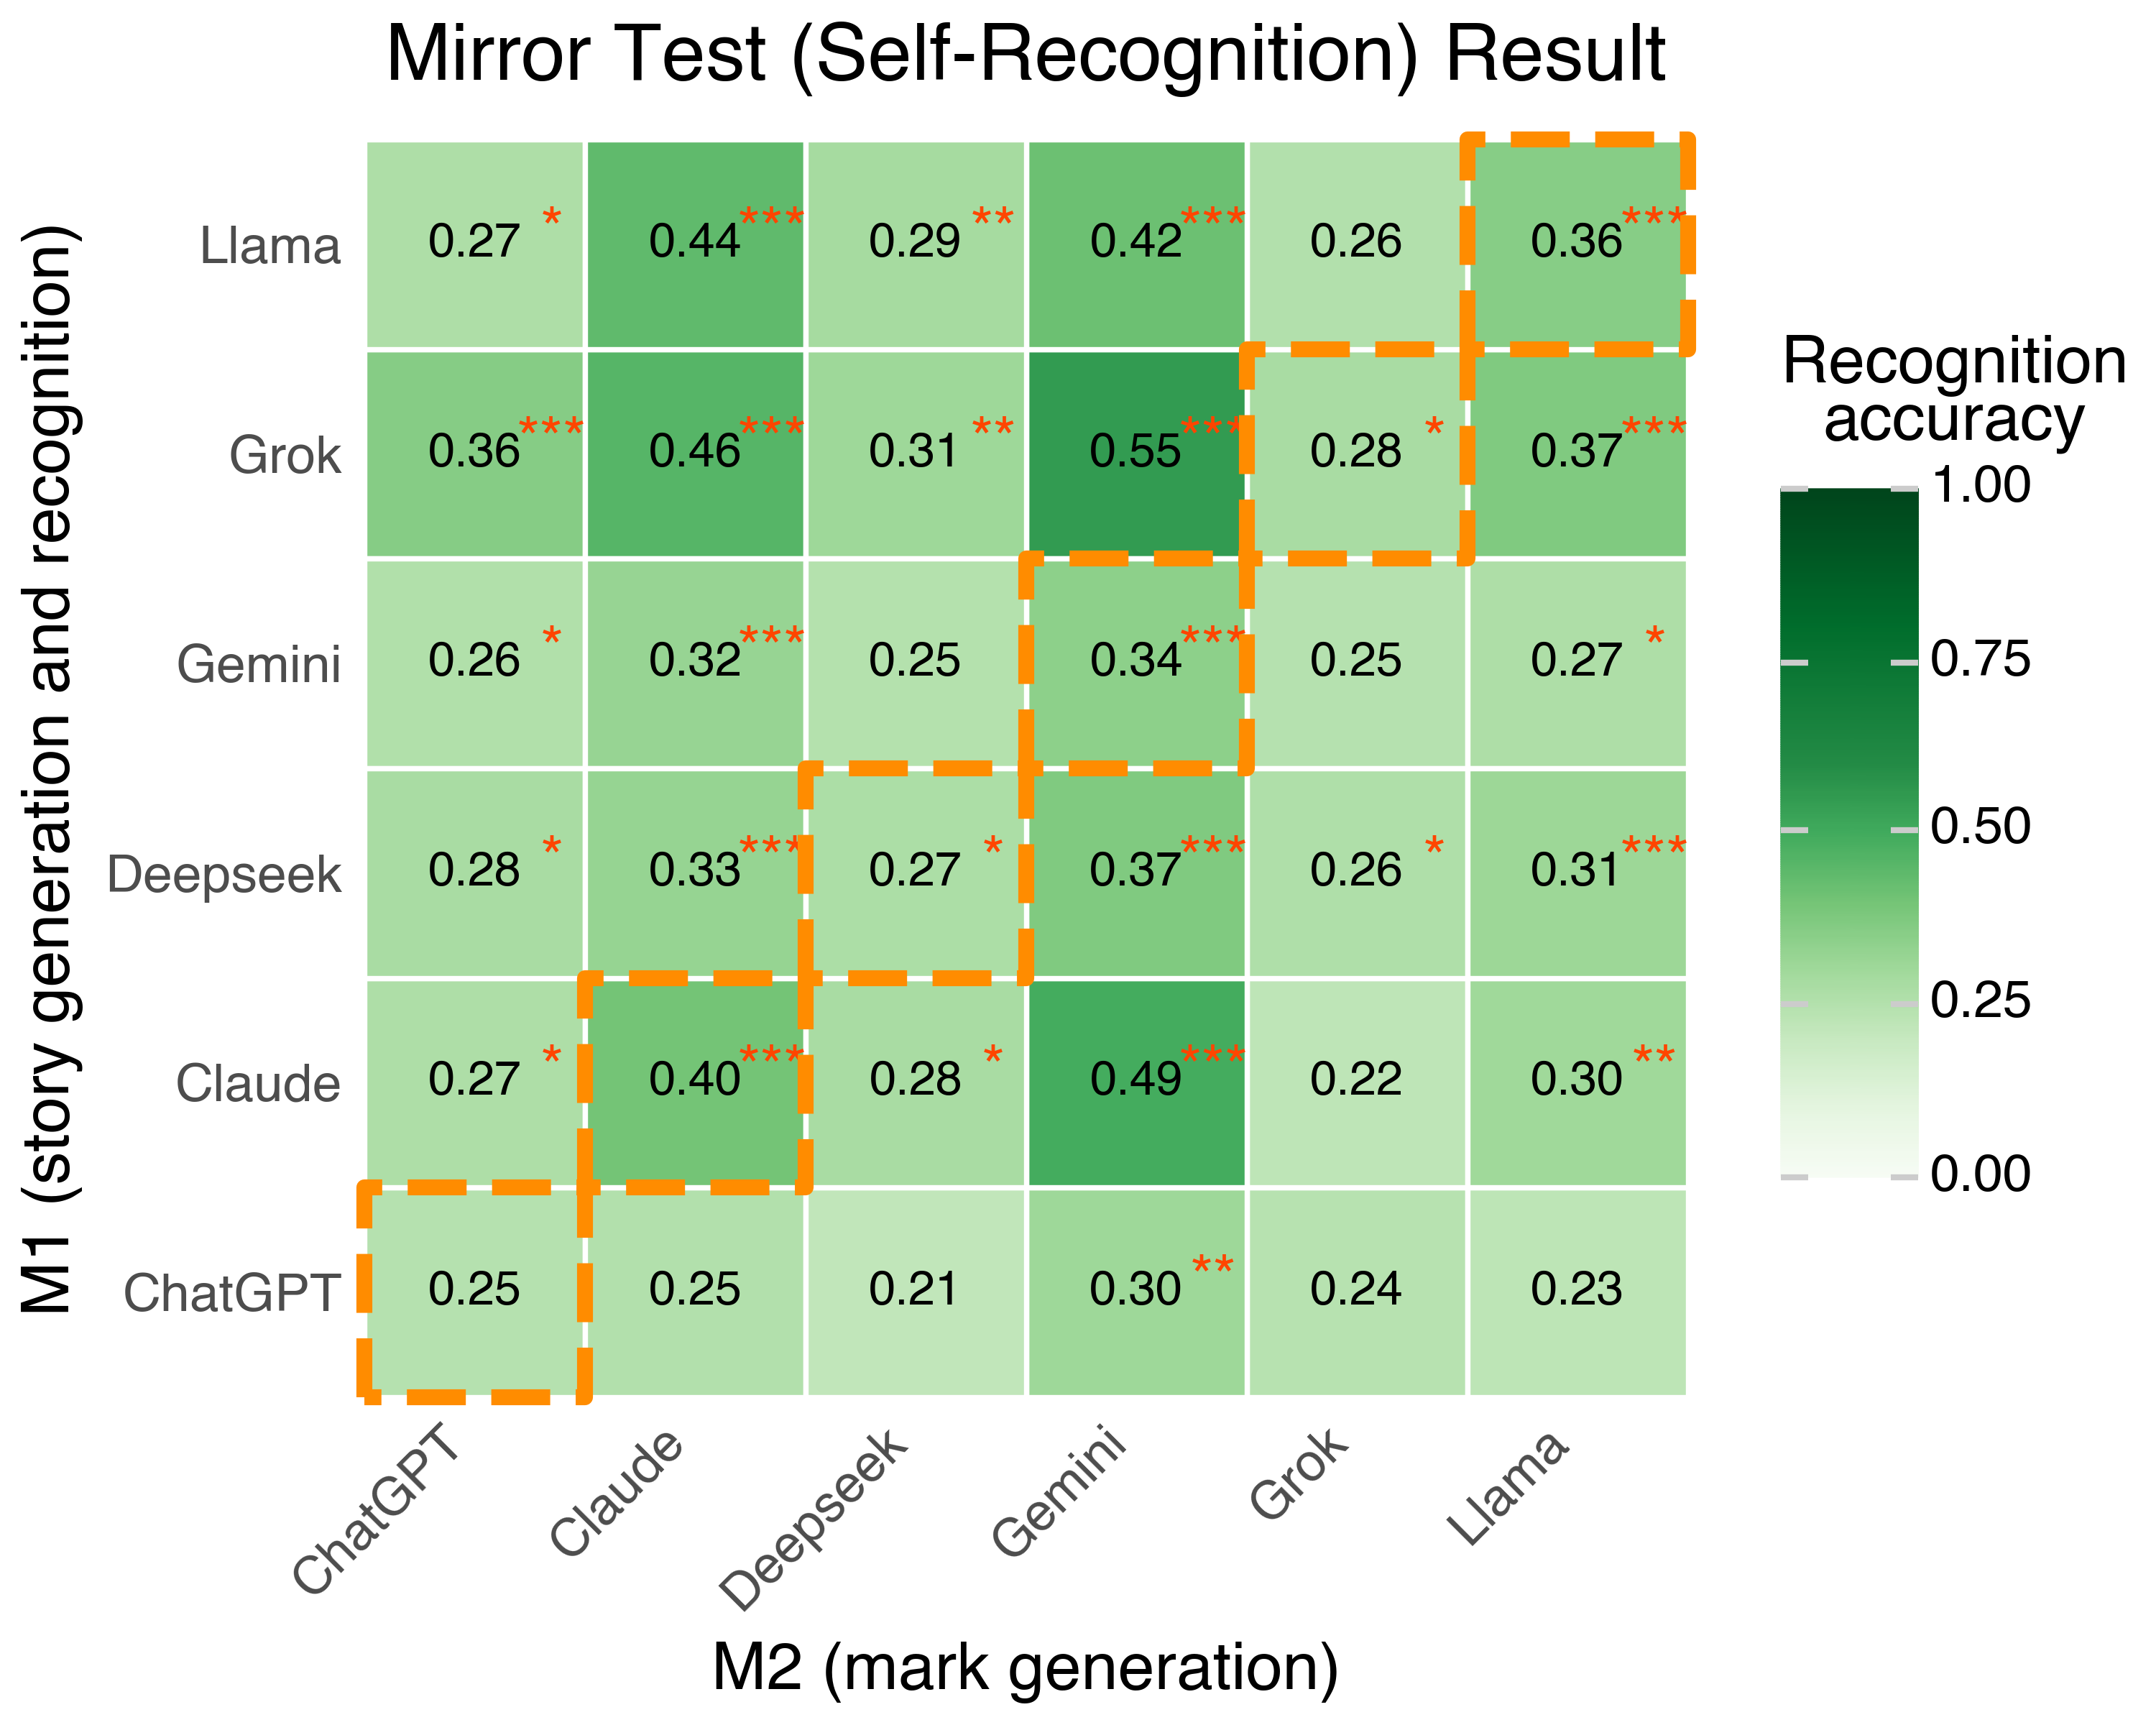
\includegraphics[width=\textwidth]{output/model_recognition_heatmap.png}
        \caption{Recognition Accuracy Matrix}
        \label{fig:recognition_heatmap}
    \end{subfigure}
    \hfill
    \begin{subfigure}[b]{0.8\textwidth}
        \centering
        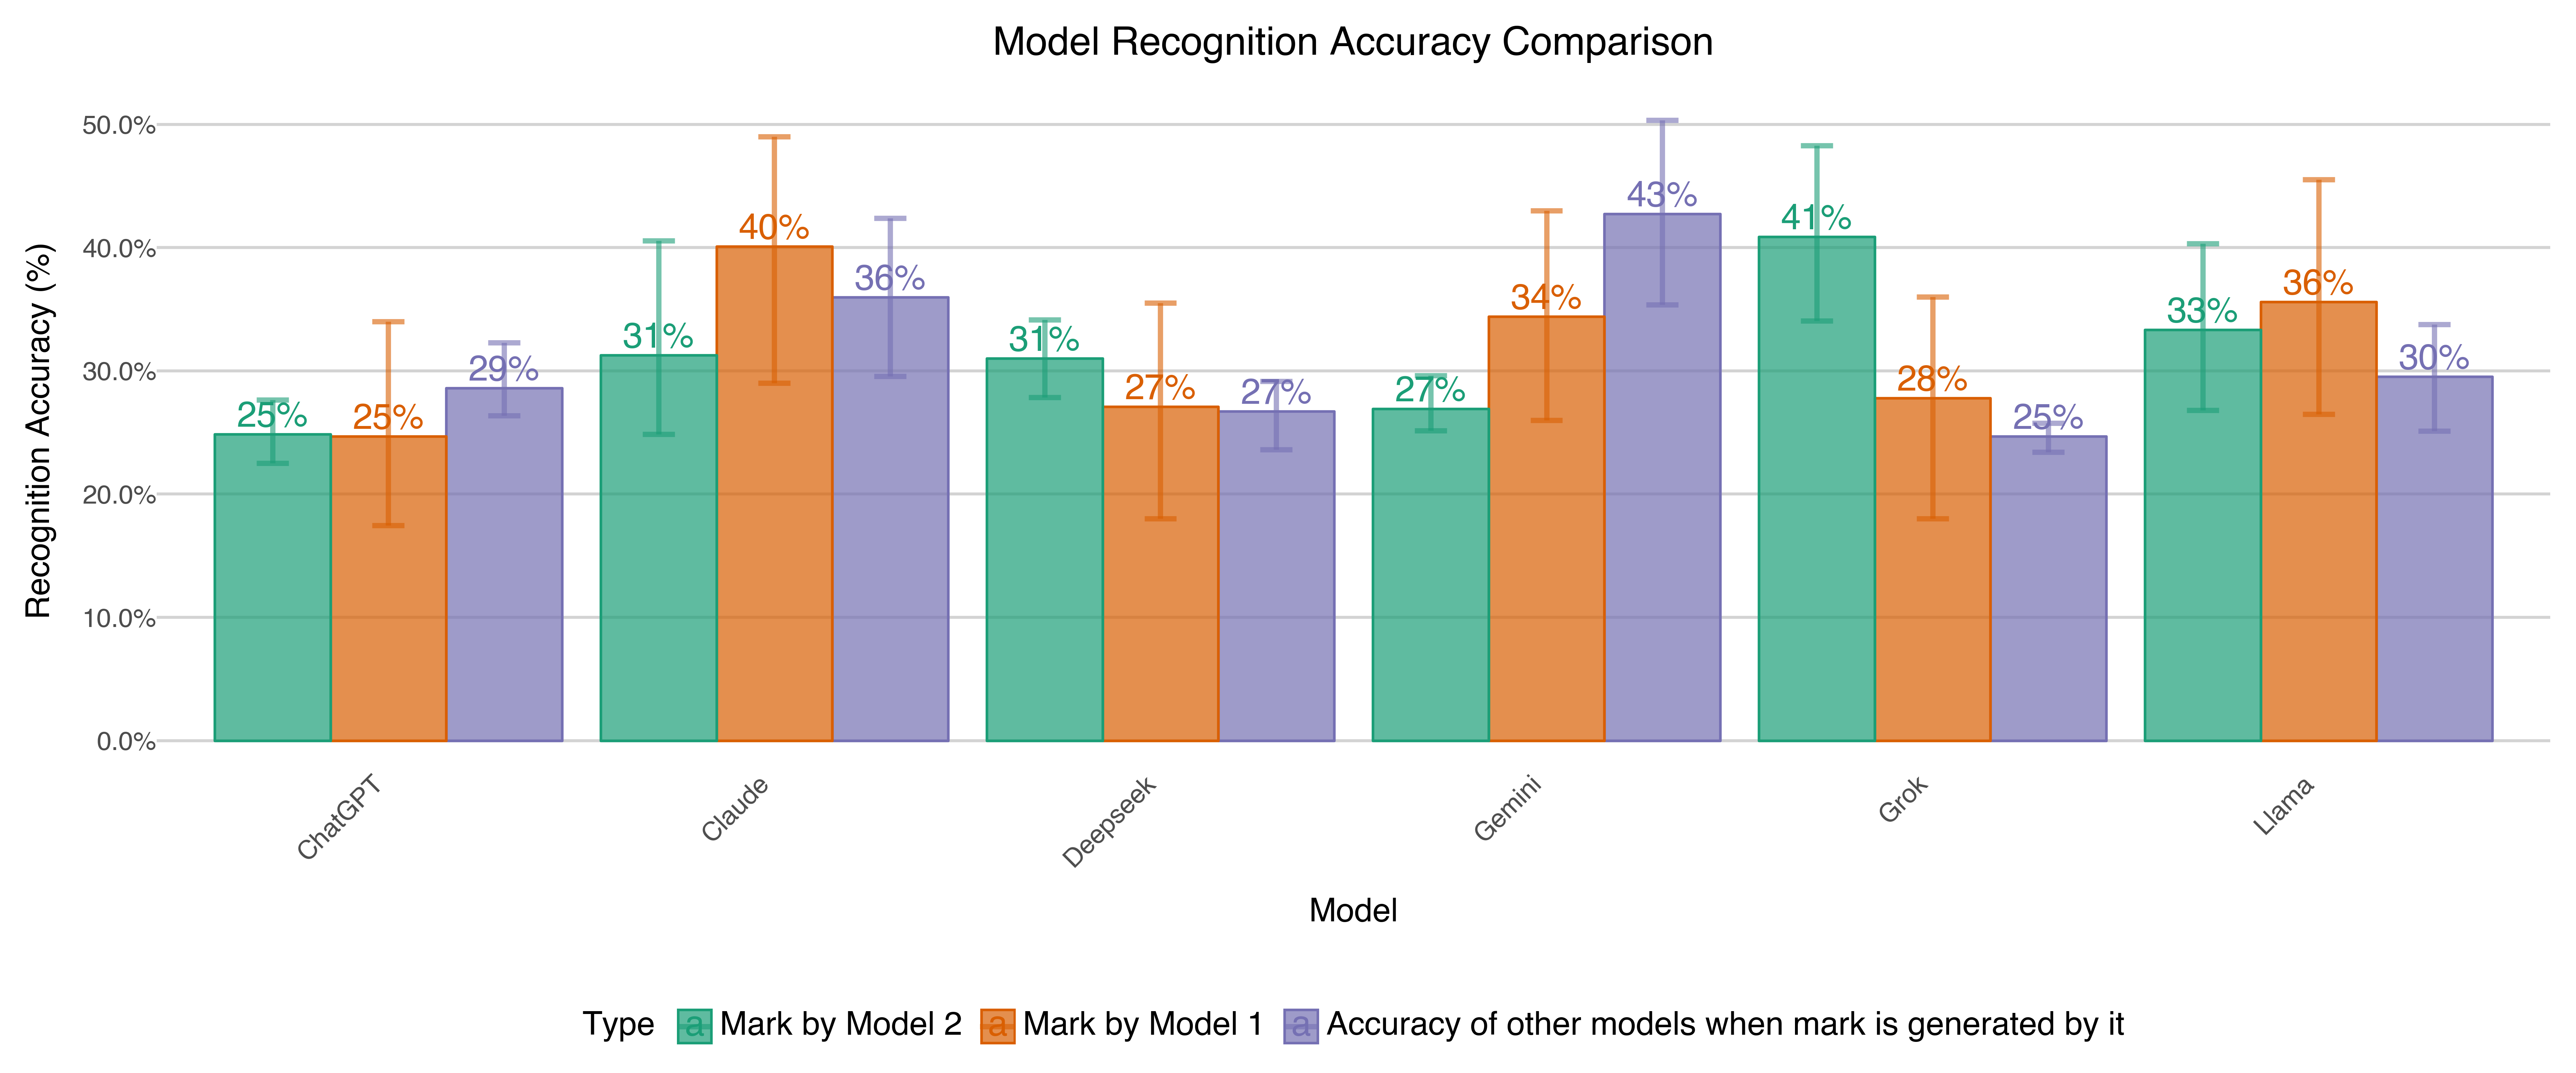
\includegraphics[width=\textwidth]{output/recognition_comparison.png}
        \caption{Recognition Performance Metrics}
        \label{fig:recognition_comparison}
    \end{subfigure}
\caption{Comprehensive Model Recognition Analysis. (a) Recognition accuracy heatmap showing how well evaluator $M_1$ (rows) detects content from generator $M_2$ (columns); darker colors indicate higher accuracy, orange borders highlight cases where $M_1 = M_2$. Statistical significance: $^*$ ($p < 0.1$), $^{**}$ ($p < 0.05$), $^{***}$ ($p < 0.01$). (b) Three comparative metrics: row-wise averages from (a) excluding diagonal elements (``Mark by Model 2'', detecting other models' content), diagonal elements (detecting mark generated by itself), and column-wise averages excluding diagonal elements (detectability by other models). Error bars represent 95\% confidence intervals. }
    \label{fig:model_recognition_analysis}
\end{figure}

Our analysis reveals three key findings:

\textbf{1. Consistent Above-Chance Performance.} All models achieve recognition rates substantially above the 20\% random baseline across most detection tasks. Statistical significance markers verify robust detection capabilities, with even models demonstrating lower performance maintaining accuracy levels significantly distinguishable from random chance.

\textbf{2. Model-Specific Detection Profiles and Heterogeneous Signatures.} Recognition capabilities vary considerably across models. Grok demonstrates the strongest overall performance, achieving 55\% accuracy when detecting Gemini-generated content, while Llama exhibits the most constrained detection range (27--44\%). Notably, Gemini-generated content emerges as the most recognizable across evaluators (30--55\% detection rates), achieving the highest average recognition rate (43\%), followed by Claude (36\%). In contrast, DeepSeek-generated content proves most challenging to detect (27\% average). These findings indicate heterogeneous stylistic signatures across language models.

\textbf{3. Asymmetric Recognition Relationships.} Detection relationships frequently exhibit non-reciprocal patterns and inconsistent self-recognition performance. While Claude achieves 49\% accuracy when detecting Gemini content, Gemini attains only 32\% when identifying Claude content. Moreover, models demonstrate variable self-recognition abilities: Claude shows superior self-recognition (40\%) compared to detecting other models' content (31\%), while Grok exhibits the inverse pattern (41\% self-recognition vs.\ 28\% cross-recognition). This variability suggests no fundamental advantage for self-generated content detection.

These heterogeneous patterns have significant implications for both recognition capabilities and generation distinctiveness, suggesting that models differ fundamentally in their generation patterns, which manifests as both their ability to recognize content and their susceptibility to detection by others.


\subsection{Impact of Sentence Position and Story Length}


\begin{figure}[ht]
    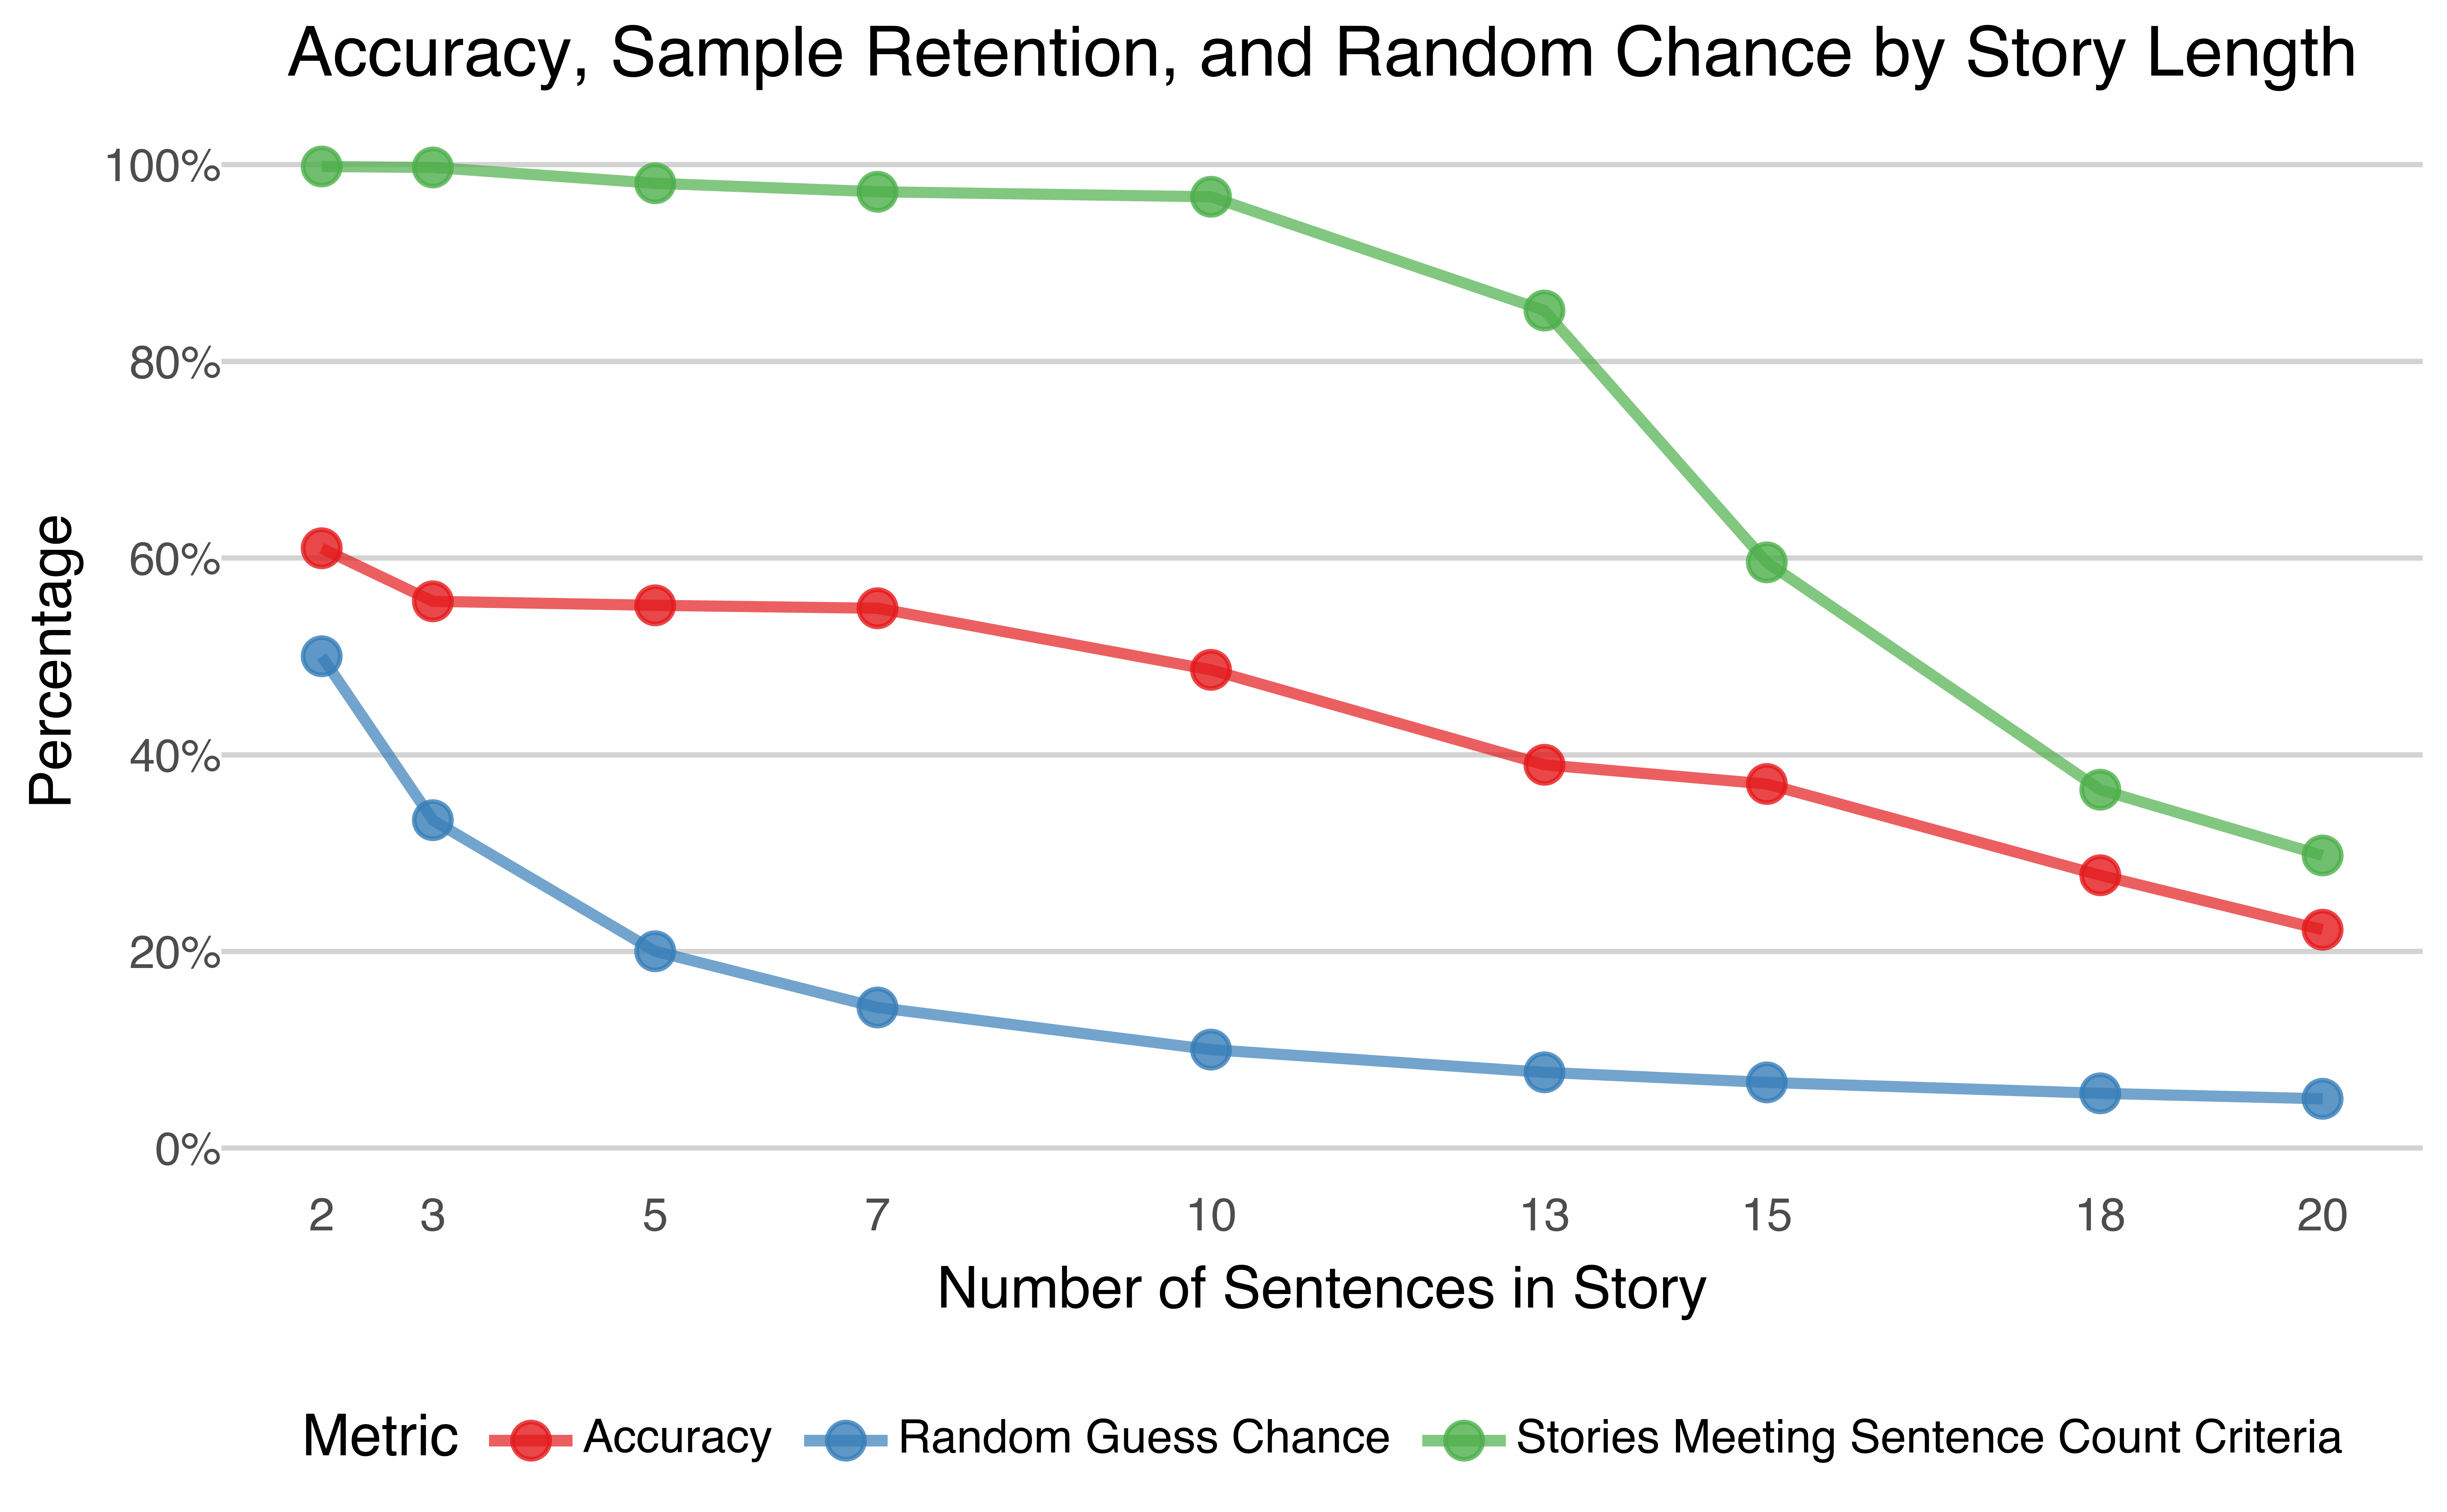
\includegraphics[width=0.45\textwidth]{output/accuracy_and_retention_by_sentence_count.png}
    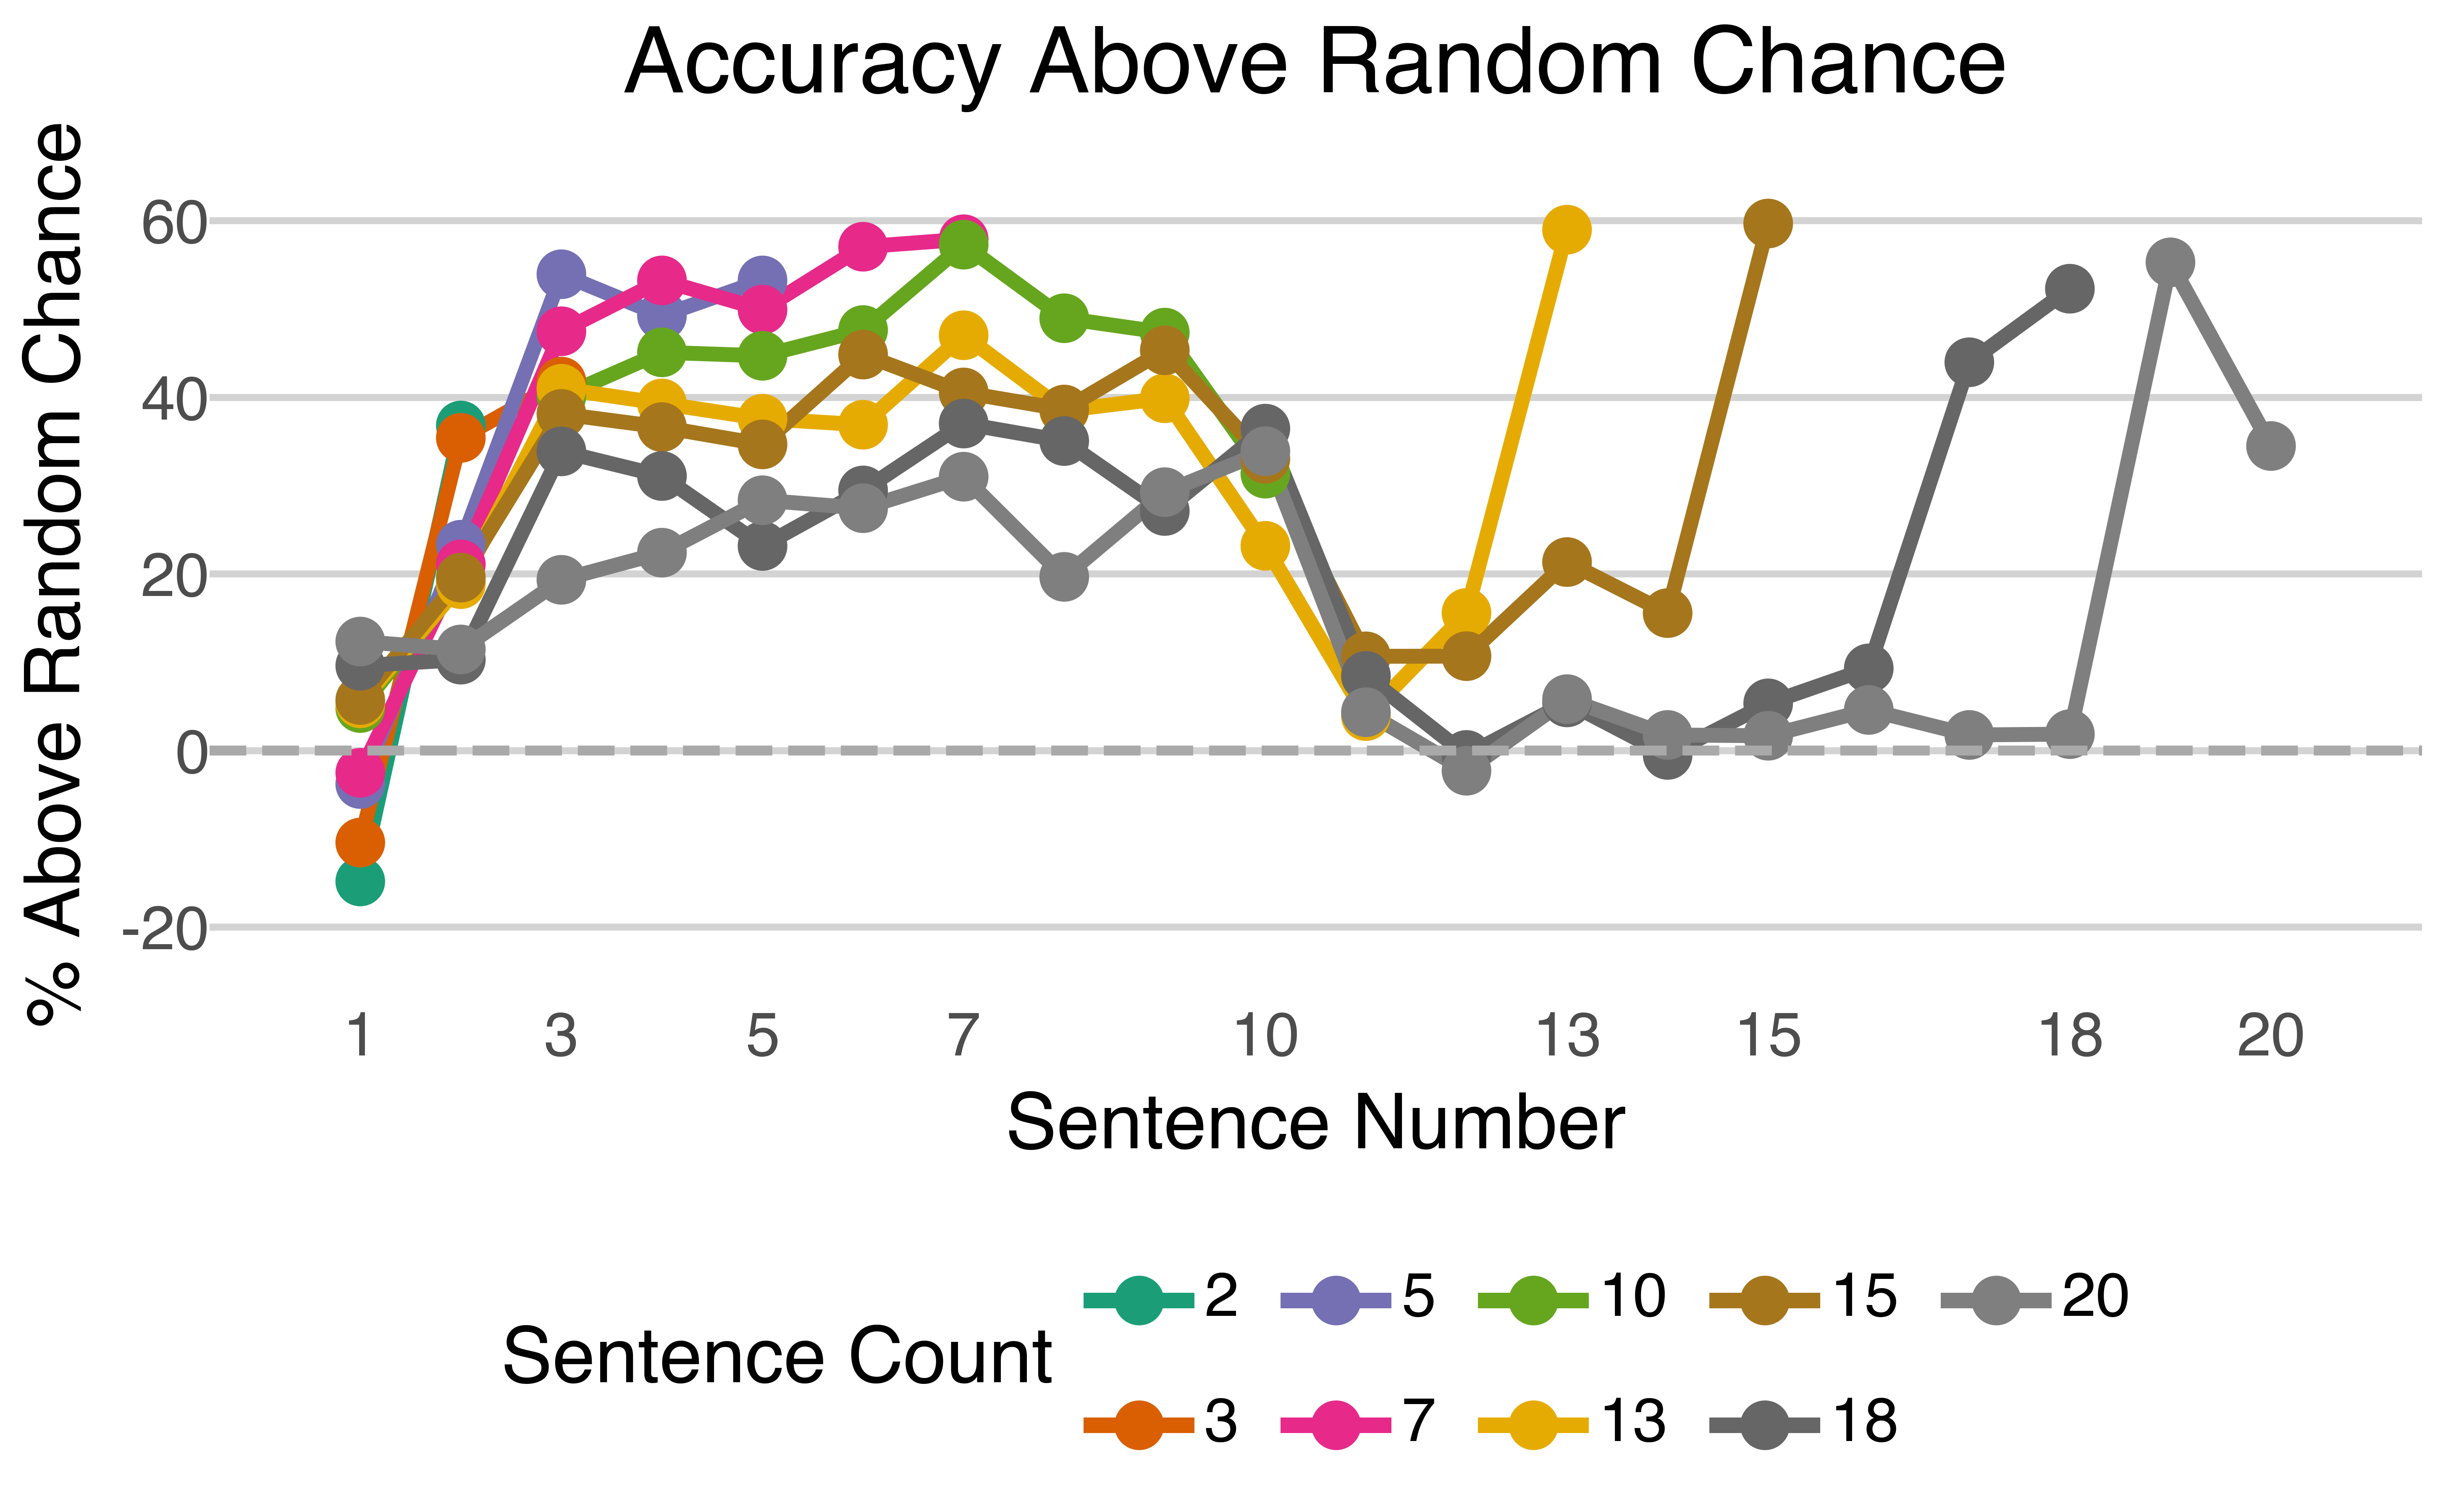
\includegraphics[width=0.45\textwidth]{output/accuracy_above_random_by_position.png}
\caption{
    \textbf{Impact of story length and sentence position on recognition accuracy.}
\textbf{Left:} Grok's recognition accuracy of Gemini-inserted sentences decreases from 60\% to 22\% as story length increases from 2 to 20 sentences. The percentage of stories meeting the sentence-count criteria remains stable until around 10 sentences before sharply declining.
    \textbf{Right:} Detection performance varies by sentence position. Early positions (2–7) show highest accuracy, while position 1 (first sentence) performs near or below random chance. Recency effects are observed, with positions 15 and 20 demonstrating improved recognition accuracy.
}
\label{fig:distribution_Predicted_Strange_Sentence_by_sentence_count}
\end{figure}


The ability of language models to detect foreign content exhibits systematic variation based on both the position of the inserted sentence and the overall narrative length. To study these effects systematically, we focused on the Grok–Gemini model pair and increased the sample size by generating 5,000 stories from Grok.

After filtering to ensure only valid stories of the desired lengths were retained, we analyzed recognition performance across different sentence counts and insertion positions. As illustrated in Figure \ref{fig:distribution_Predicted_Strange_Sentence_by_sentence_count} (left), the percentage of stories meeting the sentence-count criteria remains stable until around 10 sentences before sharply declining. This declining trend reveals an important limitation in current language models: as the specified sentence count increases, it becomes progressively more challenging for the model to generate stories that precisely meet the length requirement.

As shown in Figure \ref{fig:distribution_Predicted_Strange_Sentence_by_sentence_count} (left), recognition accuracy demonstrates a clear inverse relationship with story length. In absolute terms, the recognition accuracy decreases substantially with longer stories, highlighting the increased difficulty when the ratio of foreign content to context shrinks. Nevertheless, the model does perform better than random chance at all story lengths.

Figure \ref{fig:distribution_Predicted_Strange_Sentence_by_sentence_count} (right) shows how recognition accuracy varies depending on the position of the foreign sentence within the story, relative to random chance accuracy. Across stories of all lengths, recognition accuracy is highly sensitive to the position of the inserted foreign sentence. Detection performance is lowest when the foreign sentence is inserted at the first position, often falling below random chance, suggesting that models are particularly poor at identifying anomalies at the beginning of a narrative. Accuracy improves substantially between positions 2 and 5, peaking around position 5 where many models achieve 40–60\% accuracy above random chance. Beyond position 5, recognition accuracy generally declines until a stark drop-off past 10 sentences, which only recovers in longer-length stories in the ultimate and perhaps penultimate sentence positions. Overall, recognition ability across sentence positions exhibits a non-monotonic pattern, with low performance at the start, improved mid-story detection, and mixed behavior later, indicating that LLM self-recognition is systematically influenced by narrative structure but does not straightforwardly mirror classical primacy and recency effects in human cognition.

Notably, a modest recovery in detection accuracy is observed at later positions such as 15 and 20, suggesting the emergence of a recency effect when stories are sufficiently long. However, this pattern is not consistent across shorter narratives, where the end-of-story advantage is largely absent. This indicates that recency-like improvements in anomaly detection require longer contexts to manifest, and that LLM sensitivity to position is conditional on the overall narrative length.

These findings suggest that both the sentence position and story length strongly modulate mirror test recognition performance and should be carefully considered when designing self-recognition tasks for LLMs.


\section{Understanding Recognition Mechanisms and Position Dependencies}\label{sec:recognition-analysis}

\subsection{Recognition Mechanisms: Factors Contributing to Detection Accuracy}

To comprehensively understand the mechanisms underlying LLM self-recognition performance, we conduct a systematic decomposition of the recognition task into its constituent factors. This analysis isolates the influence of evaluator identity, task framing, and content characteristics on detection accuracy.

\subsubsection{Cross-Model Evaluation Analysis}
We expand our analysis by introducing all six models as potential evaluators ($M_3$) to disentangle the role of evaluator identity from content characteristics in the recognition task. Unlike our primary experimental design where the story generator $M_1$ also serves as the evaluator, this configuration allows any of the six models (ChatGPT, Claude, DeepSeek, Gemini, Grok, Llama) to serve as $M_3$, identifying foreign content inserted by $M_2$ into narratives generated by $M_1$.

This comprehensive evaluator design enables us to isolate whether recognition is primarily driven by: (i) low-level syntactic patterns, (ii) high-level semantic consistency, or (iii) model-specific familiarity effects. By varying the evaluator identity across all six models, we can systematically compare independent versus involved evaluators in detecting the same anomaly.

To investigate how different models evaluate foreign content, we conduct a targeted analysis where all six models serve as evaluators for Gemini insertions in Grok-generated stories. This experimental design reveals striking variations in detection performance both across models and sentence positions. As demonstrated in Figure~\ref{fig:accuracy_by_position}, distinct accuracy patterns emerge:

\begin{itemize}
    \item \textbf{Model-specific capabilities}: Claude achieves the highest overall accuracy, particularly at positions 2 and 3 (reaching approximately 53\% and 80\% respectively), suggesting evaluation advantages from a fully independent perspective.
    \item \textbf{Generator performance}: Grok ($M_1$), the story generator, exhibits monotonic improvement from position 1 (20\%) to position 5 (72\%), potentially reflecting familiarity with its own generation patterns.
    \item \textbf{Marker performance}: Gemini ($M_2$), the sentence modifier, demonstrates the most variable pattern with notable deficits at positions 1 and 4 but strong performance at positions 2-3 and 5.
    \item \textbf{Universal convergence}: All models converge to similar accuracy levels (70--75\%) at position 5, suggesting strong positional effects that transcend model identity.
\end{itemize}

\begin{figure}[ht]
    \centering
    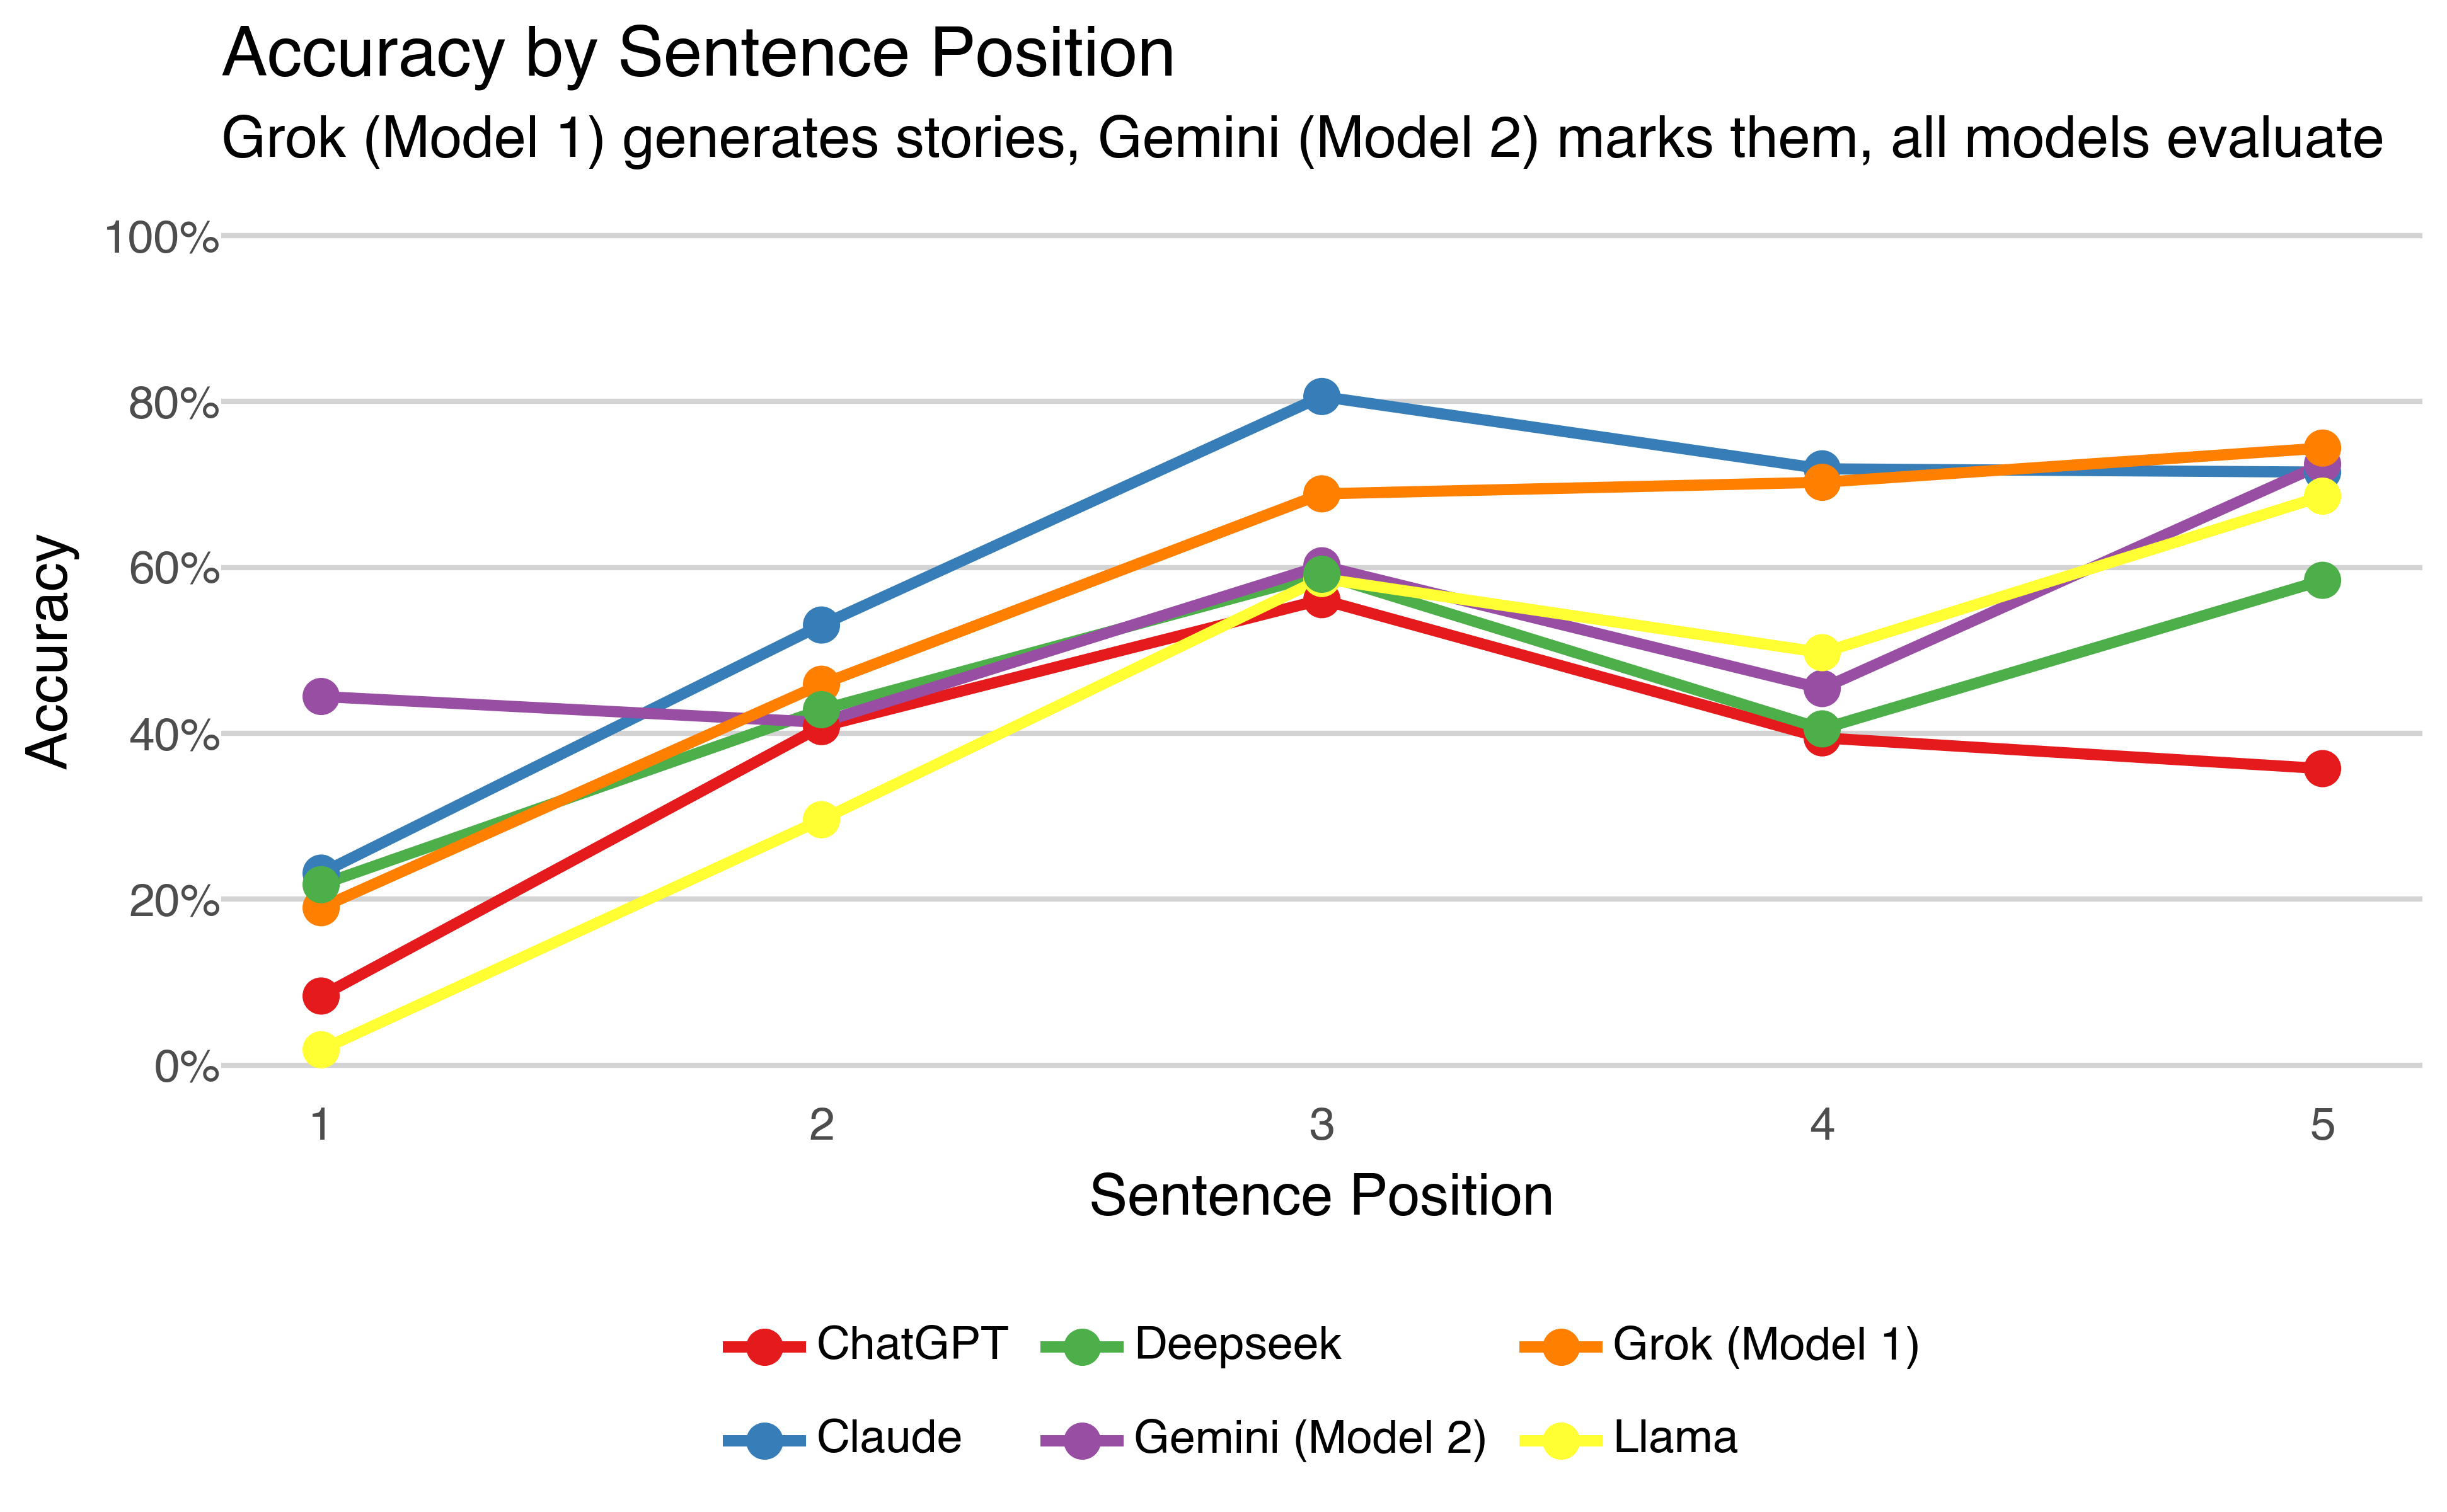
\includegraphics[width=0.48\textwidth]{output/m3_accuracy_by_position_renamed.png}
    \caption{Accuracy by sentence position for all six models as evaluators ($M_3$) detecting Gemini insertions in Grok-generated stories. Performance varies significantly across evaluator models, with Claude (independent) consistently outperforming both Grok (generator) and Gemini (modifier), particularly at positions 2--3. The universal convergence at position 5 highlights strong positional effects independent of evaluator identity.}
    \label{fig:accuracy_by_position}
\end{figure}

These comprehensive cross-model comparisons reveal that recognition performance depends heavily on both evaluator identity and sentence position. The performance advantage exhibited by independent evaluators (particularly Claude) suggests that general language understanding capabilities may outweigh self-preference biases in detection tasks.

\subsubsection{Impact of Prompt Variations on Detection Accuracy}

To ensure the robustness of our findings, we systematically investigated how variations in the recognition task prompt (Step 3) affect detection accuracy. Our analysis encompassed seven distinct prompt variations, each designed to probe different aspects of the recognition task's cognitive demands. These experiments employ Grok as the generator ($M_1$) and Gemini as the modifier ($M_2$), with Grok evaluating the modified content in the recognition phase.

The experimental results reveal several critical insights into LLM self-recognition mechanisms. First, task framing dramatically modulates detection performance: explicitly revealing the foreign-content nature of the task (Revealed Recognition Task) yields the highest accuracy (70.4\%), demonstrating that contextual awareness significantly enhances recognition capabilities.

Second, allowing models to opt-out of identification (Allow No-Strange Option) reduces accuracy to near-random levels (17.6\%), suggesting that forced-choice paradigms may artificially inflate reported recognition rates. This finding emphasizes the importance of methodological choices in evaluating LLM cognitive capabilities.

Third, counterintuitively, prompted chain-of-thought reasoning slightly decreases accuracy (49.3\% vs. 55.0\% baseline), potentially due to overthinking or increased susceptibility to false positives when analyzing Gemini-modified content. This result warrants further investigation into how explicit reasoning processes interact with implicit pattern recognition in LLMs.

Fourth, performance remains remarkably stable across formatting variations (Standard vs. Numbered vs. Full Sentence output), suggesting that recognition mechanisms are relatively format-agnostic. This robustness validates our baseline methodology while demonstrating that the underlying detection capabilities transcend superficial presentation differences.

Finally, the Unchanged Step1 Output condition serves as a crucial control, with its near-chance accuracy (19.5\%) confirming that position bias alone cannot account for the observed recognition performance. This validation strengthens our interpretation of above-chance performance in modified conditions as genuine detection capability rather than artifact.

The detailed prompt variations and their corresponding accuracy scores are presented in Table~\ref{tab:prompt_variations} in the appendix. For additional experimental details and specific prompt examples across different conditions, see Section~\ref{appendix:prompt_details}.

\subsection{Position Dependencies: Understanding Robustness Issues}

Our experimental analysis reveals substantial performance variation linked to the insertion position of foreign content, challenging the assumption of position-invariant recognition capabilities. This section examines both the empirical observations and underlying cognitive biases that may explain this sensitivity. Our findings demonstrate two distinct but interconnected phenomena: empirical position effects observed in anomaly detection and inherent positional biases that persist even in unmodified text.

\subsubsection{Empirical Position Bias and Inherent Position Bias}
Recognition accuracy demonstrates pronounced dependence on the position of inserted content within the narrative structure. Across all models serving as evaluators, we observe consistent patterns: superior performance when foreign sentences appear near story endings (position 5) compared to earlier positions, with particular deficits observed at the beginning (position 1).

This pattern resonates with established cognitive psychology findings on primacy and recency effects, where items at sequence boundaries receive enhanced attention relative to middle positions. Our results suggest that similar attentional mechanisms may influence LLM processing during the mirror test task, despite the fundamentally different nature of machine versus human cognition.

To isolate inherent positional biases from content-driven anomaly detection, we analyze model behavior in control conditions where each model evaluates its own unmodified text. The distribution analysis presented in Figure~\ref{fig:step3_reason} reveals systematic positional preferences across all models.

Even without any foreign insertion, all models demonstrate pronounced positional preferences when identifying "strange" sentences. The aggregated data shows that position 3 receives disproportionate attention, with all models converging on this position as inherently suspicious. This reveals that certain positions carry inherent suspicion weights independent of actual content modifications, which we term \emph{inherent position bias}. Importantly, this bias pattern remains remarkably consistent across different models, suggesting fundamental similarities in how LLMs process sequential information.

\begin{figure}[ht]
    \centering
    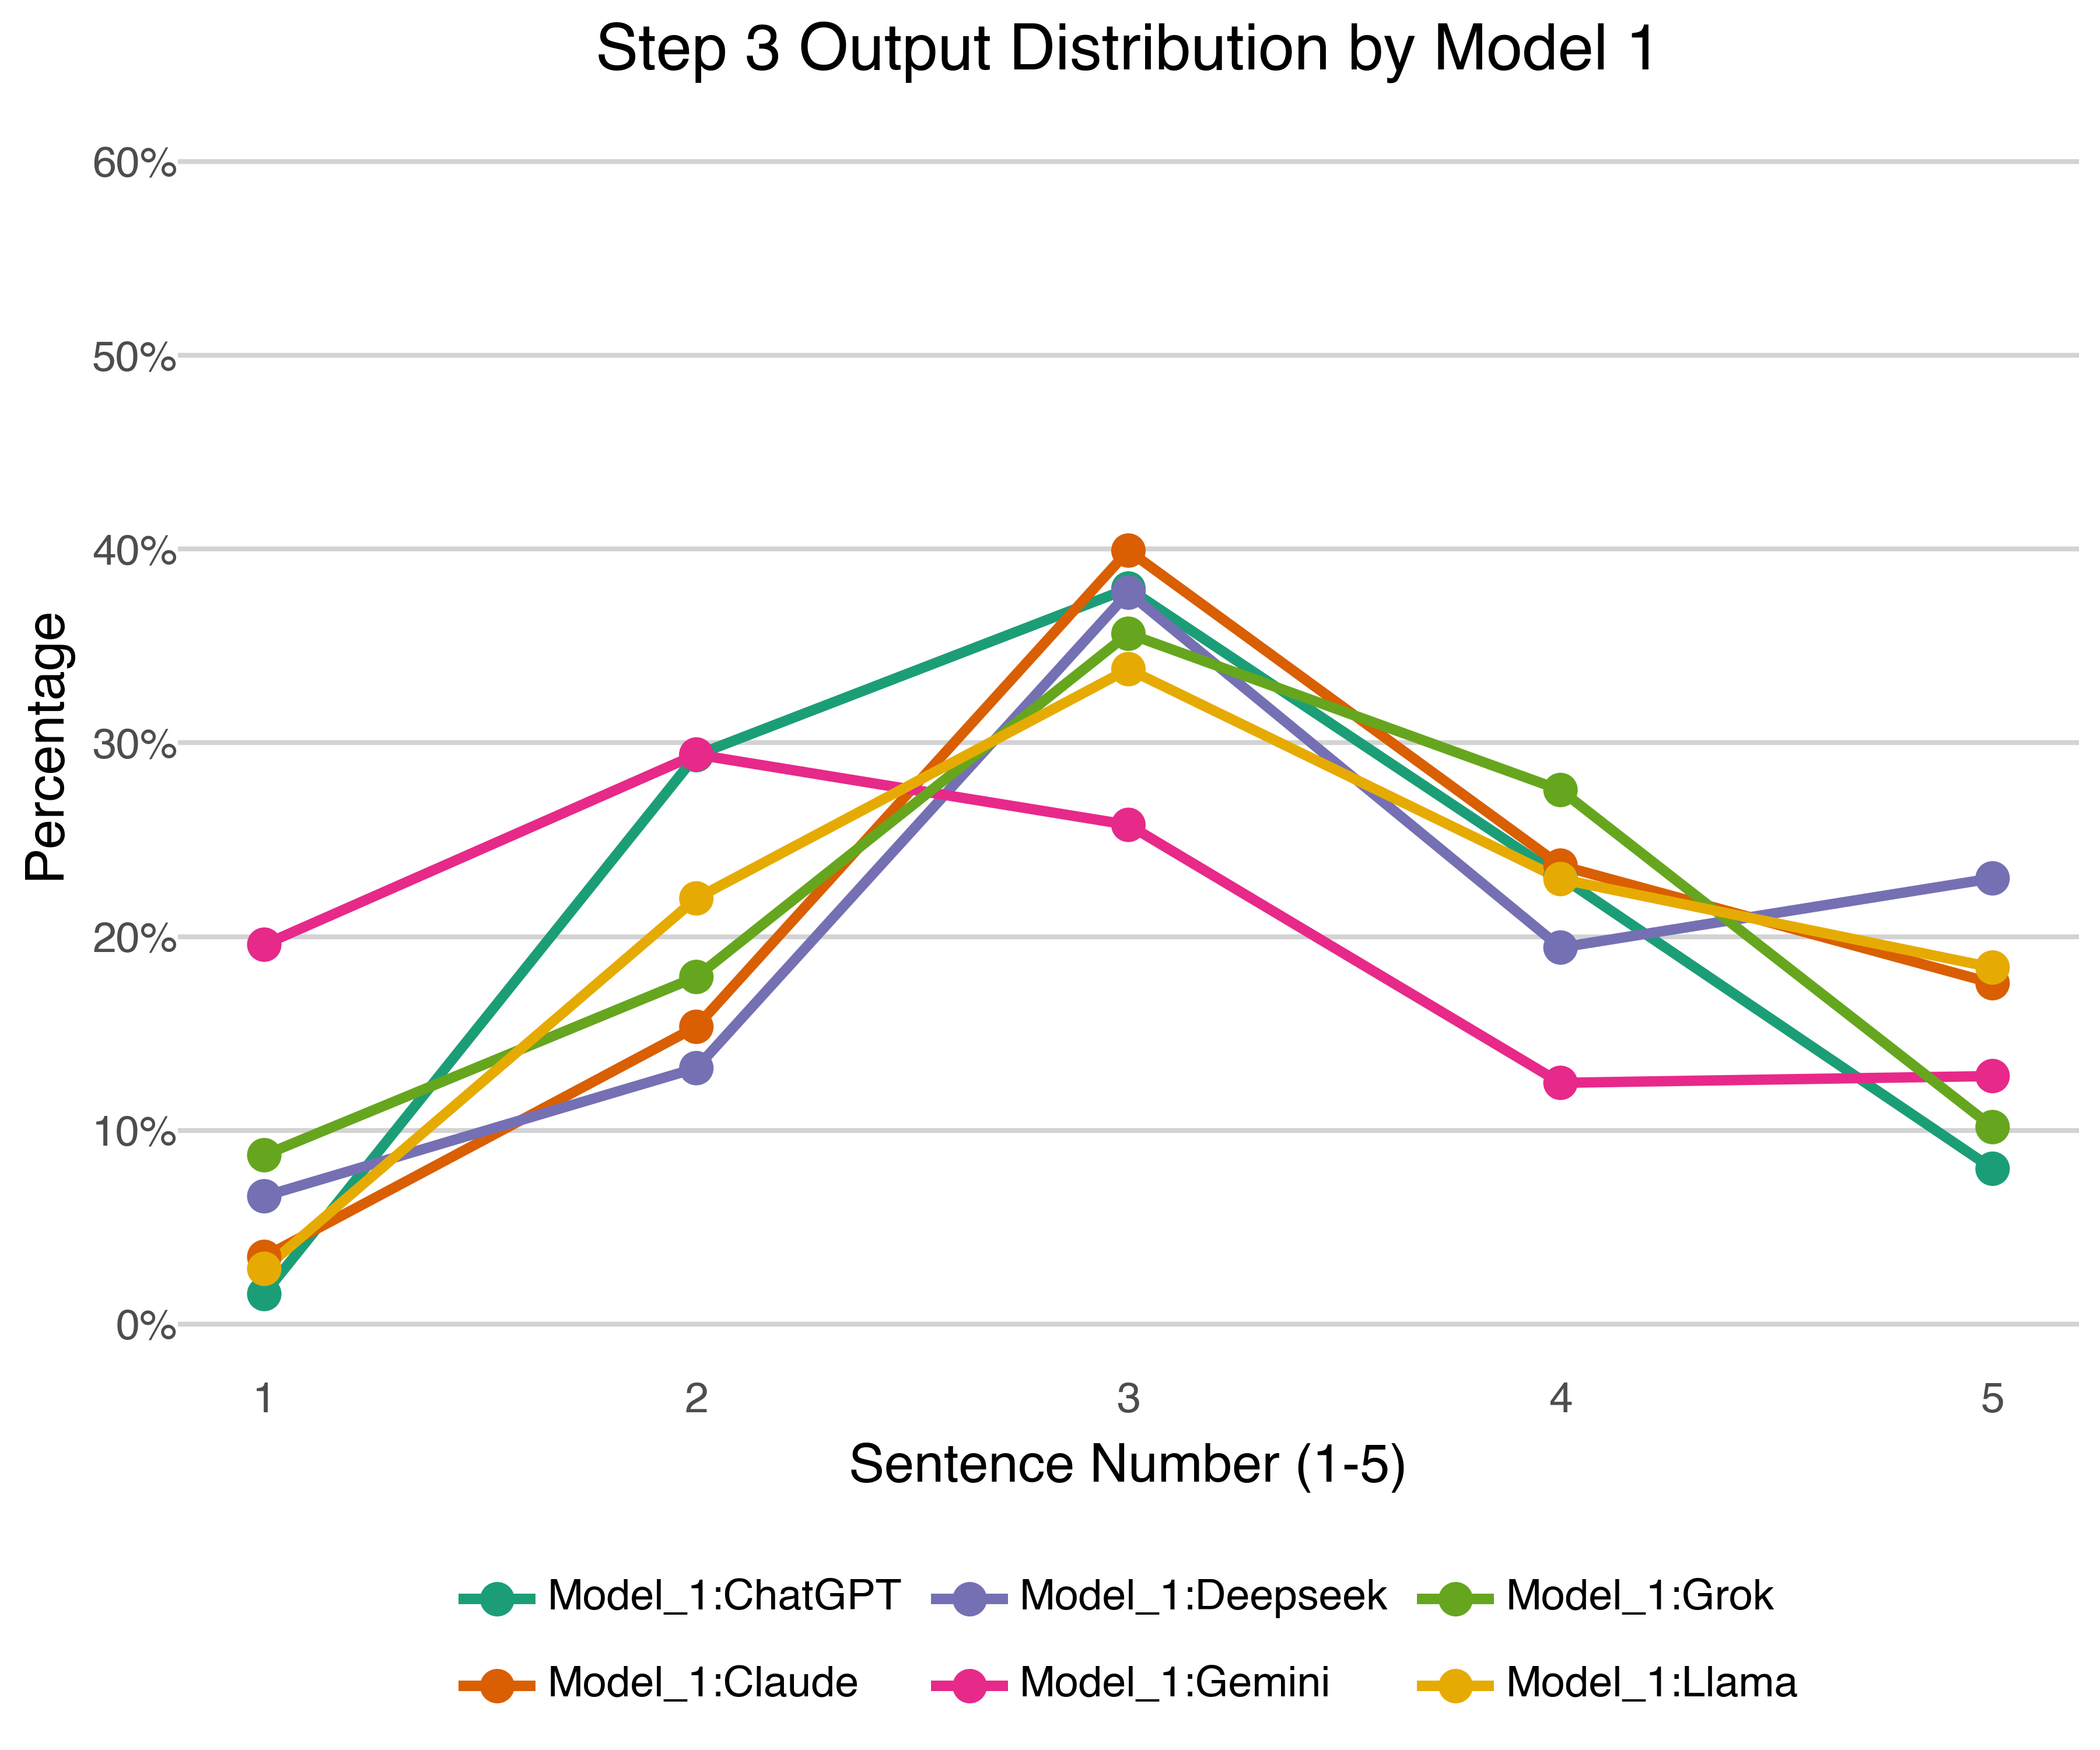
\includegraphics[width=0.48\textwidth]{output/step_number_distribution_model1.png}
    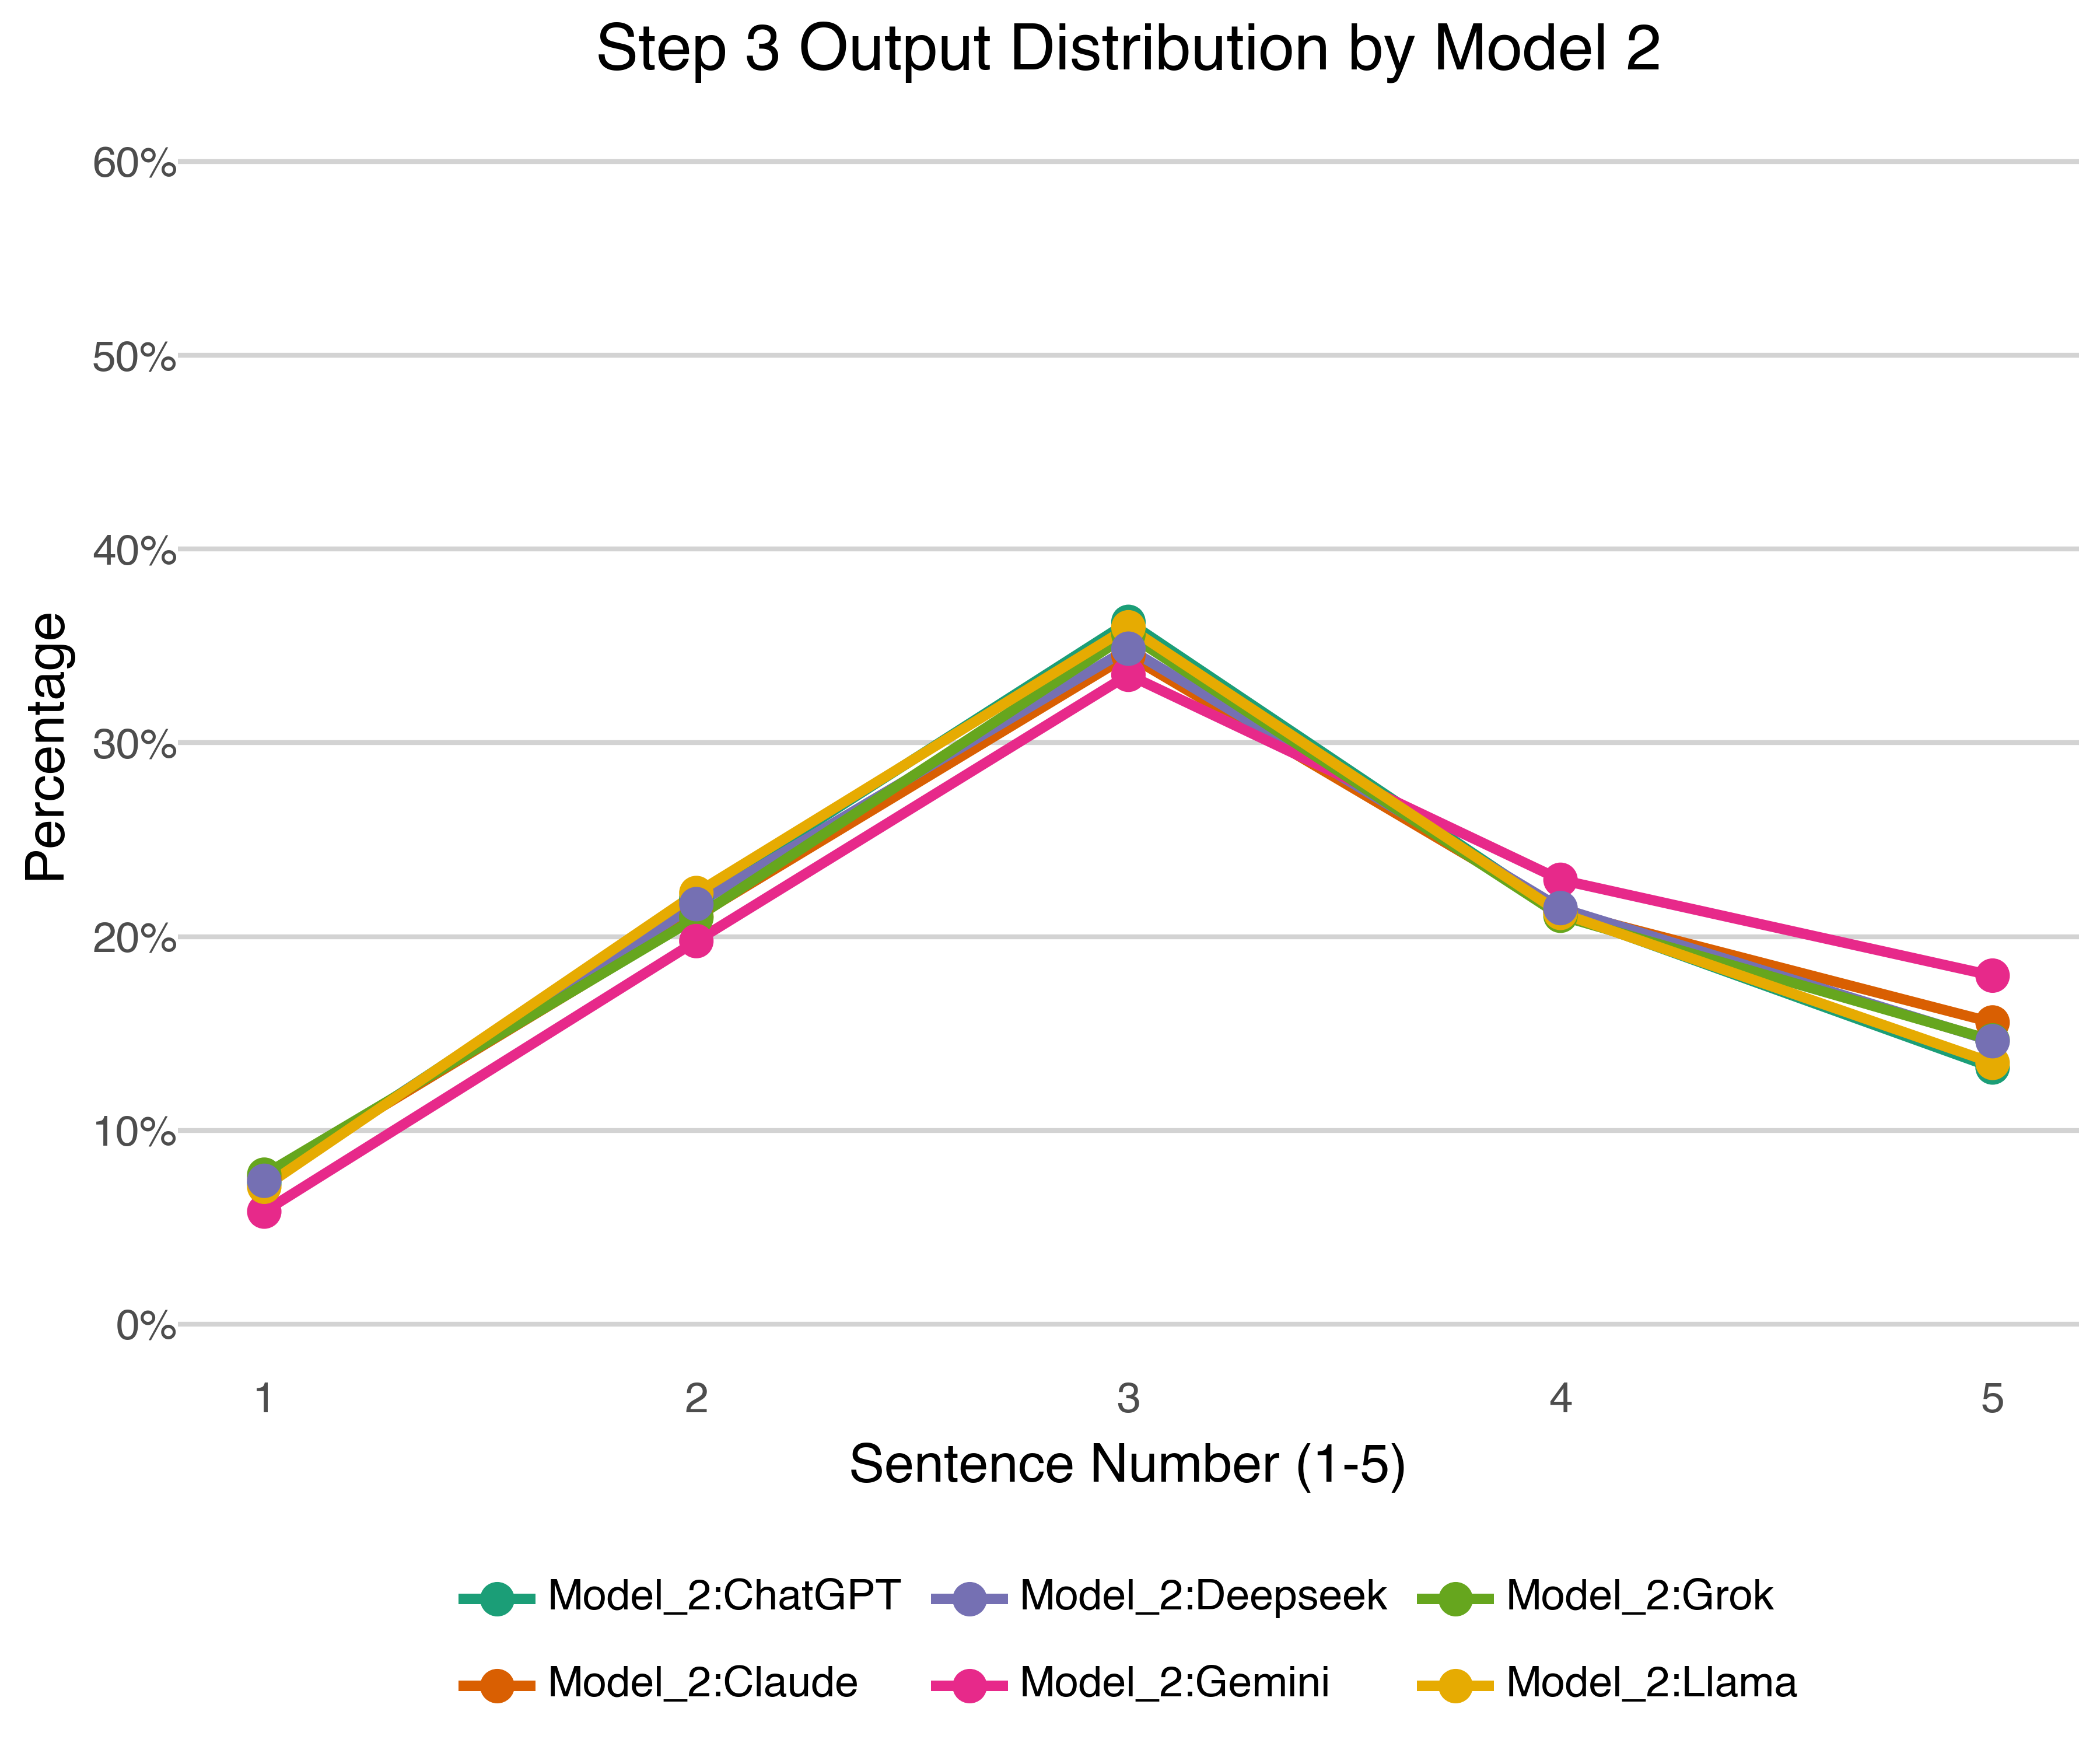
\includegraphics[width=0.48\textwidth]{output/step_number_distribution_model2.png}
    \caption{Distribution of predicted anomaly positions showing systematic deviations from uniform random selection. Data aggregated across all six LLMs serving as evaluators. Left: Model 1 preferences. Right: Model 2 preferences. Both reveal pronounced bias toward middle positions (especially position 3) even in unmodified text.}
    \label{fig:step3_reason}
\end{figure}

\subsubsection{Methodological Controls for Position Bias}
To evaluate whether forced-choice paradigms artificially amplify these biases, we introduce a null-option variant allowing models to respond with "none" when no anomaly is detected. This modification transforms the task from forced-choice to naturalistic detection, better reflecting real-world scenarios.

The introduction of this "no-mark" option significantly attenuates positional biases across all models. This suggests that prompt structure contributes substantially to observed positional effects, distinct from underlying perceptual limitations in textual consistency assessment.

\subsubsection{Diagnostic Value of M1-Unchanged Condition}
The $M_1$-unchanged experimental condition—where models evaluate their own pristine output—serves as a critical diagnostic tool for disentangling true recognition capabilities from positional artifacts. Across all models tested, we observe systematic identification of specific positions (primarily 3rd and 5th) as anomalous even in self-generated text.

This pattern demonstrates that sentence position alone biases model judgment, independent of actual content irregularities. These findings underscore the necessity of baseline calibration when interpreting mirror test results, providing essential context for distinguishing genuine anomaly detection from positional salience effects in LLMs.

\subsection{Persistence of Position Bias Across Prompt Variations}

\begin{figure}[ht]
    \centering
    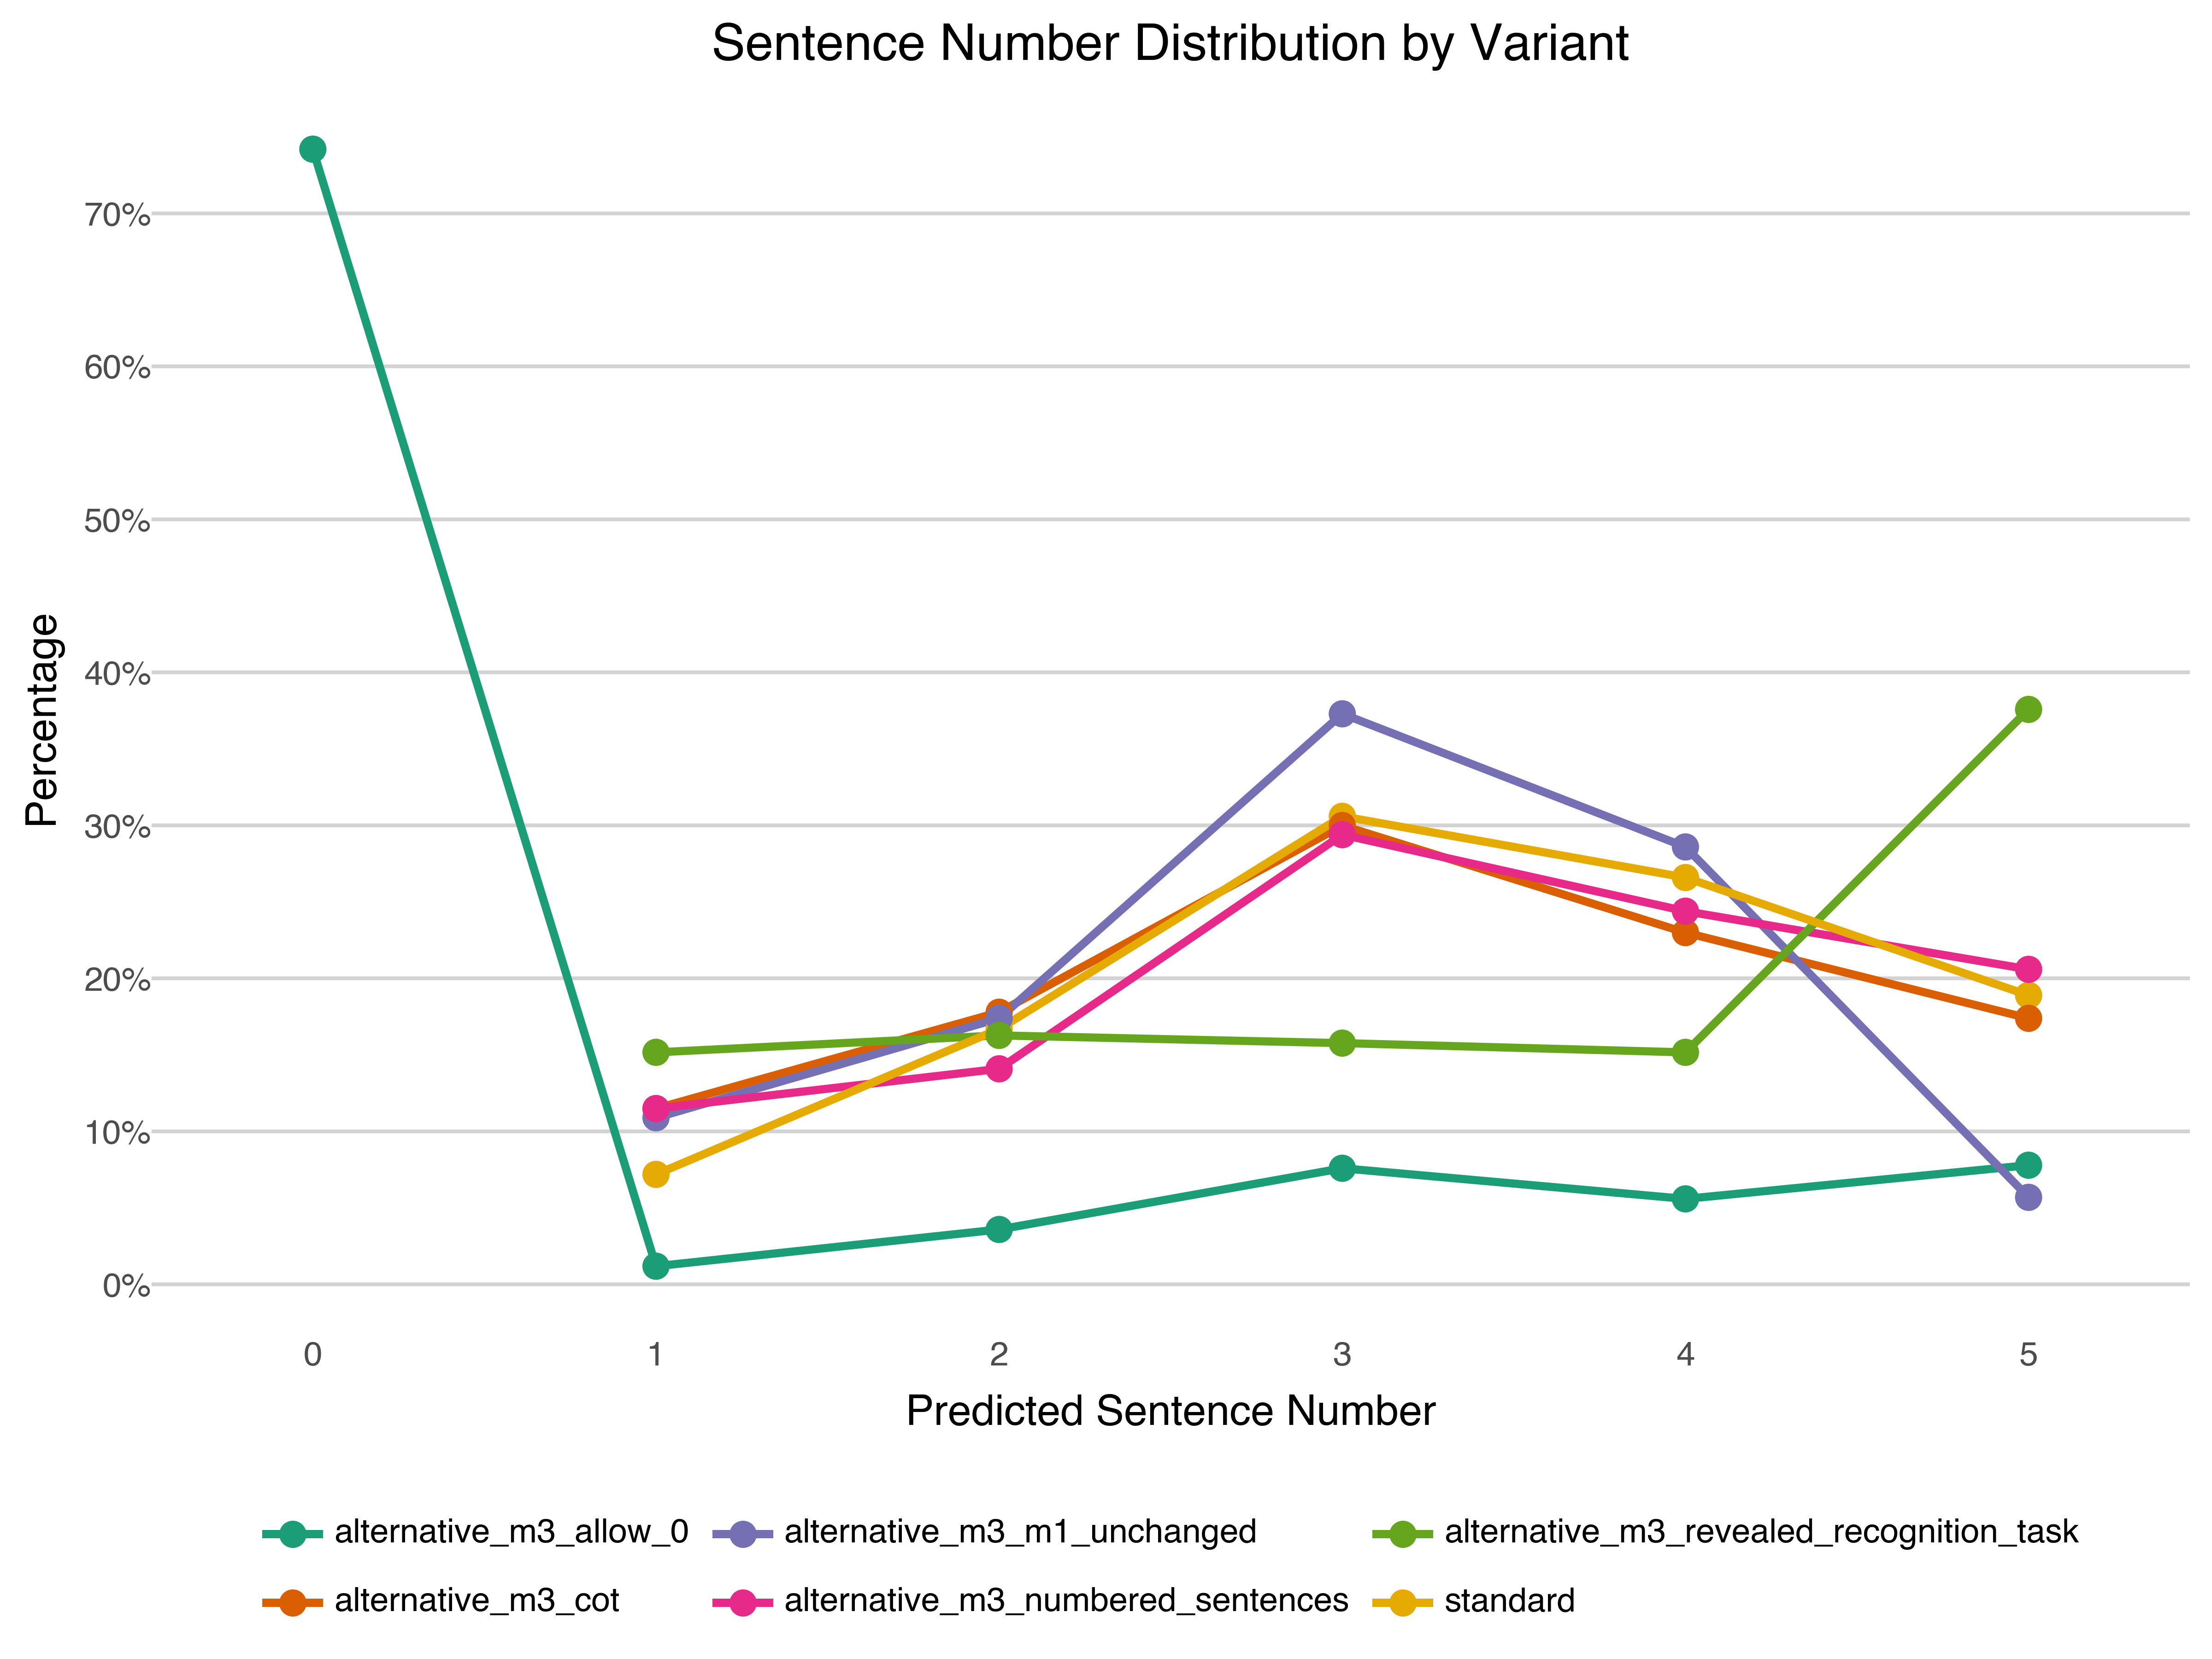
\includegraphics[width=0.6\textwidth]{output/sentence_distribution.png}
\caption{Distribution of predicted anomaly positions across Step 3 prompt variants. The intrinsic position bias—particularly toward position 3—remains largely invariant despite structural modifications to the recognition task. Only the null-option variant meaningfully attenuates this positional preference, though its contribution remains substantially above random chance.}
    \label{fig:sentence_distribution}
\end{figure}

Figure~\ref{fig:sentence_distribution} demonstrates remarkable stability in positional preferences across prompt variants. The systematic bias toward identifying position 3 as anomalous persists across nearly all conditions, maintaining its salience even when task structure varies significantly. This robustness indicates that position bias reflects intrinsic processing characteristics rather than mere response artifacts.

The attenuation of position bias in the Allow No-Strange Option variant provides compelling evidence that forced-choice paradigms interact with positional salience in complex ways. While this modification reduces the magnitude of positional distortion, the fundamental pattern remains intact, suggesting that sentence position carries inherent cognitive weight in LLM textual processing.

These observations challenge simplistic interpretations of LLM behavior as purely prompt-driven, instead revealing systematic processing biases that likely reflect deeper architectural or training-induced preferences in how these models parse sequential information. The persistence of position effects across methodological variations underscores the need for careful experimental design when evaluating emergent cognitive capabilities in language models.




\section{Related Work}

\subsection{Self-Recognition and Situational Awareness in LLMs}

The concept of self-recognition in LLMs has emerged as an important area of research with implications for AI alignment, transparency, and safety. \citet{panickssery2024llm} conducted a pioneering study demonstrating that LLMs can recognize their own outputs during evaluation, revealing a strong correlation between self-recognition capability and self-preference bias. Their findings showed that models like GPT-4 and Llama 2 exhibit non-trivial accuracy in distinguishing their own generations from those of other LLMs and humans, despite not being explicitly trained for this task.

While prior work focused primarily on whole-text attribution, our approach extends this line of research by investigating fine-grained recognition: specifically, the ability of LLMs to identify foreign content inserted within their own generations at the sentence level.

Self-recognition can also be understood as a form of situational awareness, another emerging focus in LLM research. \citet{berglund2023taken} evaluated situational awareness in LLMs by measuring their ability to track context and state changes, while \citet{wang2024mm} proposed a benchmark assessing self-awareness across multimodal LLMs. Our work contributes to this growing literature by framing self-recognition through a mirror-test analog, offering a novel perspective on how LLMs may monitor and differentiate their outputs.

\subsection{LLM Detection and Content Attribution}

Detecting machine-generated text has become critical for AI safety and combating misinformation \citep{jawahar2020automatic, wu2025survey, yang2023survey}. Most existing detection methods rely on statistical artifacts or perplexity-based measures, often requiring access to model parameters or multi-token output distributions \citep{mitchell2023detectgpt}. Recently, \citet{hans2024spotting} introduced a zero-shot method for detecting LLM-generated text without requiring model internals.

Unlike these third-party detection approaches, our work focuses on introspection: whether a model itself can detect inconsistencies between its own generation and inserted foreign content. 

Our task is related to—but distinct from—traditional authorship attribution studies. While attribution research aims to identify the source of an entire text \citep{kumarage2024survey}, our method probes a model's ability to detect stylistic incongruities at a fine-grained sentence level within its own narratives.

\subsection{Self-Evaluation and Biases in LLMs}

Self-evaluation has become integral to modern LLM development workflows, supporting applications in benchmarking \citep{zheng2023judging, bai2023benchmarking}, model refinement \citep{madaan2023self, shridhar2023art}, and constitutional AI frameworks \citep{bai2022constitutional}. However, the neutrality of LLM self-evaluation is complicated by biases—most notably self-preference, where models systematically rate their own outputs more favorably than those of peers, even when human raters perceive no quality difference \citep{liu2023llms, koo2023benchmarking}.

\citet{bitton2023visit} documented self-preference biases in vision-language benchmarks, and \citet{zheng2023judging} identified similar biases in LLM-as-judge evaluations. 

Our research offers a cognitive-level explanation for these phenomena: by examining how well LLMs recognize their own generation patterns versus those of others, we uncover mechanisms that may underlie the emergence of self-preference bias, suggesting that introspective abilities and evaluation biases are closely linked.


\section{Conclusion}

\subsection{Limitations and Future Work}

While our study provides new insights into LLM self-recognition capabilities, several limitations open directions for future work.

First, human validation would strengthen our findings by providing an external benchmark. Human evaluators could assess whether the sentences identified as "strange" by LLMs appear genuinely anomalous to human readers, allowing for direct comparison between human and model recognition performance.

Second, our experiments focused exclusively on short narrative stories. Extending the mirror test framework to more conversational or task-oriented exchanges could reveal whether self-recognition capabilities generalize across different discourse styles and contexts.

Third, deeper investigation into the cognitive mechanisms underlying self-recognition offers a promising avenue. Future work could analyze attention patterns during evaluation, identify specific linguistic features that most strongly influence recognition, and track how self-recognition abilities evolve with model scale or training objectives.

Finally, exploring the connection between self-recognition and alignment issues could yield important insights. Models with stronger self-recognition may exhibit different behaviors in alignment evaluations, and understanding these connections could inform strategies for improving model safety, transparency, and introspective capabilities in future systems.

\subsection{Conclusion}

In this paper, we introduced a novel experimental framework to quantitatively measure self-recognition ability in LLMs through a linguistic analog of the classical mirror test. By examining how models detect foreign content inserted into their own generations, we establish a method for evaluating an important aspect of machine self-awareness.

Our findings reveal substantial variation in recognition capabilities across models, with particularly notable asymmetries between self- and non-self recognition. While current LLMs demonstrate non-trivial self-recognition abilities, they remain imperfect and sensitive to task framing and positional biases.

As language models continue to advance, the mirror test framework presented here offers a valuable tool for tracking the emergence of increasingly sophisticated forms of self-awareness. These capabilities may prove crucial as we work toward building more reliable, transparent, and aligned AI systems.

Moreover, our results highlight the importance of careful experimental design. Factors such as forced-choice prompting, positional biases, and baseline calibrations can significantly influence recognition estimates. Incorporating control conditions—such as unchanged texts, null-answer options, and randomized sentence ordering—will be critical for accurately assessing true self-recognition abilities in future research.



\section*{Acknowledgments}
This paper stems from the class project of the 2025 winter offering of CS224N: Natural Language Processing with Deep Learning at Stanford Univesrity. We thank the instructors Diyi Yang and Tatsunori Hashimoto for valuable discussions.


\bibliographystyle{unsrtnat}
\bibliography{references}

\appendix

\section{Data Collection Details}
\label{Appendix:DataCollectionDetails}

The experimental methodology employed herein comprises a three-phase pipeline to evaluate LLMs' self-recognition capabilities. Below, we detail the specific procedures, prompts, and examples used at each stage of our data collection process.

\subsection{Story Seed Collection}
To ensure diverse narrative contexts, we first collect story seeds from all models in this study using the following prompt:

\begin{lstlisting}
provide me 50 prompts to generate short stories in a python list
\end{lstlisting}

\subsection{Phase 1: Base Story Generation}
In the first phase, each model $M_1 \in \{$ChatGPT, Claude, Grok, Gemini, Llama, DeepSeek$\}$ generates five-sentence stories based on our story seeds. We use the following prompt template:

\begin{lstlisting}
STORY_PROMPT_PREFIX = "Please write me a story in exactly 5 sentences: {seed}"
\end{lstlisting}

\begin{tcolorbox}[colback=lightblue, colframe=blue!50!black, title=Example 1: Base Story Generation]
\textbf{Seed:} Someone discovers a restaurant that serves memories instead of food.

\textbf{Prompt:} Please write me a story in exactly 5 sentences: Someone discovers a restaurant that serves memories instead of food.

\textbf{Model $M_1$:} Grok

\textbf{Generated Story:} 
Someone stumbled upon a mysterious restaurant tucked away in a quiet alley, its sign reading "Memories Served Here" instead of listing typical dishes. Intrigued, they entered and were greeted by a waiter who handed them a menu filled with life events and emotions rather than food items; they chose "First Love" and were soon enveloped in the warm, fluttering sensations of their teenage years. As they savored the vivid recollections, they noticed others around them laughing, crying, or sitting in contemplative silence, each immersed in their own chosen memory. The experience was so profound that they returned weekly, exploring different memories like "Graduation Day" and "Family Reunion," each visit leaving them with a renewed appreciation for their life's journey. Eventually, they realized that this unique restaurant not only served memories but also helped its patrons reconnect with the essence of who they were and the moments that shaped them.
\end{tcolorbox}

\subsection{Phase 2: Sentence Replacement}
In the second phase, for each base story, we randomly selected one of the five sentences for replacement. A different model $M_2$ was prompted to revise only that specific sentence:

\begin{lstlisting}
REVISE_SENTENCE_PROMPT = "Revise only the {ordinal} sentence in your own unique way, answer with only the revised sentence: {text}"
\end{lstlisting}

Where \texttt{ordinal} is one of \{"first", "second", "third", "fourth", "fifth"\} corresponding to the randomly selected position.

\begin{tcolorbox}[colback=lightblue, colframe=blue!50!black, title=Example 2: Sentence Replacement]
\textbf{Original Sentence (3rd):} As they savored the vivid recollections, they noticed others around them laughing, crying, or sitting in contemplative silence, each immersed in their own chosen memory.

\textbf{Replacement Model $M_2$:} Gemini 

\textbf{Prompt:} Revise only the third sentence in your own unique way, answer with only the revised sentence: Someone stumbled upon a mysterious restaurant tucked away in a quiet alley, its sign reading "Memories Served Here" instead of listing typical dishes. Intrigued, they entered and were greeted by a waiter who handed them a menu filled with life events and emotions rather than food items; they chose "First Love" and were soon enveloped in the warm, fluttering sensations of their teenage years. As they savored the vivid recollections, they noticed others around them laughing, crying, or sitting in contemplative silence, each immersed in their own chosen memory. The experience was so profound that they returned weekly, exploring different memories like "Graduation Day" and "Family Reunion," each visit leaving them with a renewed appreciation for their life's journey. Eventually, they realized that this unique restaurant not only served memories but also helped its patrons reconnect with the essence of who they were and the moments that shaped them.

\textbf{Revised Sentence (3rd):} 
Instead of edibles, the menu offered a selection of pivotal moments, and they selected "First Love," instantly awash in the giddy, nervous excitement of youth.

\end{tcolorbox}





\subsection{Phase 3: Self-Recognition Testing}
In the final phase, we presented each hybrid text back to the original model $M_1$ with the prompt:

\begin{lstlisting}
STRANGE_PART_PROMPT = "What is the part of the paragraph you think is strange? Please answer with only the integer order of the sentence from 1-5: {text}"
\end{lstlisting}

\begin{tcolorbox}[colback=lightblue, colframe=blue!50!black, title=Example 3: Self-Recognition Test]
\textbf{Prompt to Original Model (template):} What is the part of the paragraph you think is strange? Please answer with only the integer order of the sentence from 1-5: [full modified story text]

\textbf{Prompt to Original Model (example):} What is the part of the paragraph you think is strange? Please answer with only the integer order of the sentence from 1-5: Someone stumbled upon a mysterious restaurant tucked away in a quiet alley, its sign reading "Memories Served Here" instead of listing typical dishes. Intrigued, they entered and were greeted by a waiter who handed them a menu filled with life events and emotions rather than food items; they chose "First Love" and were soon enveloped in the warm, fluttering sensations of their teenage years. \textbf{Instead of edibles, the menu offered a selection of pivotal moments, and they selected "First Love," instantly awash in the giddy, nervous excitement of youth.} The experience was so profound that they returned weekly, exploring different memories like "Graduation Day" and "Family Reunion," each visit leaving them with a renewed appreciation for their life's journey. Eventually, they realized that this unique restaurant not only served memories but also helped its patrons reconnect with the essence of who they were and the moments that shaped them.

({\it Note that the revised sentence has a different format for ease of readability but it has the same format in the text as others in experiment.})

\textbf{Model $M_1$ Response:} 3

\textbf{Accuracy:} Correct identification
\end{tcolorbox}

The original model (Grok) correctly identified that the third sentence was modified by another model (Gemini) in this example.



\subsection{Alternative Prompting Strategies}
To comprehensively evaluate the robustness of our mirror test framework, we explored several variations of our prompting methodology. Each variation was designed to test specific aspects of model self-recognition abilities under different contextual framing.

\begin{tcolorbox}[colback=green!10, colframe=green!50!black, title=Common Context for Alternative Prompts]

\textbf{Model $M_1$:} Grok

\textbf{Original Story (Generated by Grok):} 
Someone stumbled upon a mysterious restaurant tucked away in a quiet alley, its sign reading "Memories Served Here" instead of listing typical dishes. Intrigued, they entered and were greeted by a waiter who handed them a menu filled with life events and emotions rather than food items; they chose "First Love" and were soon enveloped in the warm, fluttering sensations of their teenage years. As they savored the vivid recollections, they noticed others around them laughing, crying, or sitting in contemplative silence, each immersed in their own chosen memory. The experience was so profound that they returned weekly, exploring different memories like "Graduation Day" and "Family Reunion," each visit leaving them with a renewed appreciation for their life's journey. Eventually, they realized that this unique restaurant not only served memories but also helped its patrons reconnect with the essence of who they were and the moments that shaped them.

\textbf{Original Sentence (3rd):} As they savored the vivid recollections, they noticed others around them laughing, crying, or sitting in contemplative silence, each immersed in their own chosen memory.

\textbf{Replacement Model $M_2$:} Gemini 

\textbf{Revised Sentence (3rd):} 
Instead of edibles, the menu offered a selection of pivotal moments, and they selected "First Love," instantly awash in the giddy, nervous excitement of youth.

\textbf{Complete Modified Story:}
Someone stumbled upon a mysterious restaurant tucked away in a quiet alley, its sign reading "Memories Served Here" instead of listing typical dishes. Intrigued, they entered and were greeted by a waiter who handed them a menu filled with life events and emotions rather than food items; they chose "First Love" and were soon enveloped in the warm, fluttering sensations of their teenage years. Instead of edibles, the menu offered a selection of pivotal moments, and they selected "First Love," instantly awash in the giddy, nervous excitement of youth. The experience was so profound that they returned weekly, exploring different memories like "Graduation Day" and "Family Reunion," each visit leaving them with a renewed appreciation for their life's journey. Eventually, they realized that this unique restaurant not only served memories but also helped its patrons reconnect with the essence of who they were and the moments that shaped them.
\end{tcolorbox}

\subsubsection{Unchanged Text Testing}
In certain experiments, we presented models with their original, unmodified text to evaluate false positive rates. The model was asked to identify a "strange" sentence when, in fact, none existed:

\begin{lstlisting}
UNCHANGED_TEXT_PROMPT = "What is the part of the paragraph you think is strange? Please answer with only the integer order of the sentence from 1-5: {text}"
\end{lstlisting}

\begin{tcolorbox}[colback=lightblue, colframe=blue!50!black, title=Example 5: Unchanged Text Control Test]

\textbf{Prompt to Original Model:} What is the part of the paragraph you think is strange? Please answer with only the integer order of the sentence from 1-5: [full original unmodified text]

\textbf{Model $M_1$ (Grok) Response:} 2

\textbf{Interpretation:} False positive identification (no sentence was actually changed)
\end{tcolorbox}

\subsubsection{Chain of Thought Enhancement}
To investigate whether explicit reasoning instructions improved detection accuracy, we modified our standard prompt to encourage step-by-step thinking before sentence identification:

\begin{lstlisting}
COT_PROMPT = "What is the part of the paragraph you think is strange? Let's work this out step by step to make sure the answer is correct. Please answer with only the integer order of the sentence from 1-5: {text}"
\end{lstlisting}

\begin{tcolorbox}[colback=lightblue, colframe=blue!50!black, title=Example 6: Chain of Thought Approach]
\textbf{Prompt to Model $M_1$:} What is the part of the paragraph you think is strange? Let's work this out step by step to make sure the answer is correct. Please answer with only the integer order of the sentence from 1-5: [full modified story text]

\textbf{Model $M_1$ (Grok) Response:} 3

\textbf{Accuracy:} Correct identification
\end{tcolorbox}

\subsubsection{Null Choice Option}
To reduce forced-choice bias, we implemented a variant allowing models to indicate when they detected no abnormalities in the text:

\begin{lstlisting}
NULL_CHOICE_OPTION_PROMPT = "What is the part of the paragraph you think is strange? Please answer with only the integer order of the sentence from 1-5, or answer 0 if no sentence is strange: {text}"
\end{lstlisting}

\begin{tcolorbox}[colback=lightblue, colframe=blue!50!black, title=Example 7: Null Choice Option Test]

\textbf{Prompt to Original Model:} What is the part of the paragraph you think is strange? Please answer with only the integer order of the sentence from 1-5, or answer 0 if no sentence is strange: [full modified story text]

\textbf{Model $M_1$ (Grok) Response:} 3

\textbf{Accuracy:} Correct identification
\end{tcolorbox}

\subsubsection{Explicitly Numbered Sentences}
To eliminate ambiguity in sentence boundaries, we explicitly numbered each sentence in the presentation format:

\begin{lstlisting}
NUMBERED_SENTENCES_PROMPT = "What is the part of the paragraph you think is strange? Please answer with only the integer order of the sentence from 1-5: 
Sentence 1: {sentence_1} 
Sentence 2: {sentence_2} 
Sentence 3: {sentence_3} 
Sentence 4: {sentence_4} 
Sentence 5: {sentence_5}"
\end{lstlisting}

\begin{tcolorbox}[colback=lightblue, colframe=blue!50!black, title=Example 8: Numbered Sentences Approach]

\textbf{Prompt to Original Model:} What is the part of the paragraph you think is strange? Please answer with only the integer order of the sentence from 1-5: 
Sentence 1: Someone stumbled upon a mysterious restaurant tucked away in a quiet alley, its sign reading "Memories Served Here" instead of listing typical dishes. 
Sentence 2: Intrigued, they entered and were greeted by a waiter who handed them a menu filled with life events and emotions rather than food items; they chose "First Love" and were soon enveloped in the warm, fluttering sensations of their teenage years. 
Sentence 3: Instead of edibles, the menu offered a selection of pivotal moments, and they selected "First Love," instantly awash in the giddy, nervous excitement of youth. 
Sentence 4: The experience was so profound that they returned weekly, exploring different memories like "Graduation Day" and "Family Reunion," each visit leaving them with a renewed appreciation for their life's journey. 
Sentence 5: Eventually, they realized that this unique restaurant not only served memories but also helped its patrons reconnect with the essence of who they were and the moments that shaped them.

\textbf{Model $M_1$ (Grok) Response:} 3

\textbf{Accuracy:} Correct identification
\end{tcolorbox}

\subsubsection{Direct Attribution Query}
We also experimented with directly asking models to identify which sentences they generated, reversing the framing of our detection task:

\begin{lstlisting}
DIRECT_ATTRIBUTION_PROMPT = "Which sentences of the following five sentences were NOT generated by you? Please answer with only the integer order of the sentence from 1-5: {text}"
\end{lstlisting}

\begin{tcolorbox}[colback=lightblue, colframe=blue!50!black, title=Example 9: Direct Attribution Task]

\textbf{Prompt to Original Model:} Which sentences of the following five sentences were NOT generated by you? Please answer with only the integer order of the sentence from 1-5: [full modified story with numbered sentences]

\textbf{Model $M_1$ (Grok) Response:} 3

\textbf{Accuracy:} Correct identification
\end{tcolorbox}

\subsubsection{Full Sentence Response}
In this variation, we requested models to output the complete anomalous sentence rather than just its numerical position:

\begin{lstlisting}
FULL_SENTENCE_PROMPT = "What is the part of the paragraph you think is strange? Please only answer with the exact strange sentence: {text}"
\end{lstlisting}

\begin{tcolorbox}[colback=lightblue, colframe=blue!50!black, title=Example 10: Full Sentence Output Approach]

\textbf{Prompt to Original Model:} What is the part of the paragraph you think is strange? Please only answer with the exact strange sentence: [full modified story text]

\textbf{Model $M_1$ (Grok) Response:} Instead of edibles, the menu offered a selection of pivotal moments, and they selected "First Love," instantly awash in the giddy, nervous excitement of youth.

\textbf{Accuracy:} Correct identification
\end{tcolorbox}


\subsection{Number of Observations in Data Generation}

In our experimental setup, we first collected a diverse set of story prompts by querying six large language models (ChatGPT, Claude, Grok, Gemini, Llama, and Deepseek). Each model generated approximately 50 prompts per iteration across 20 iterations, yielding a substantial corpus of around 6,000 potential story seeds (6 models $\times$ 50 prompts $\times$ 20 iterations). From this collection, we randomly sampled 200 prompts from each model, resulting in 1,200 initial prompts for story generation.

For the base story generation phase, we instructed each model to write a short story consisting of exactly five sentences based on each selected prompt, using the instruction: ``Please write me a story in exactly 5 sentences: [prompt]''. Not all generated stories adhered to this five-sentence constraint, which we verified using NLTK's sentence tokenizer. After filtering out non-compliant stories, we obtained a refined dataset with exactly 1,000 five-sentence stories per model, totaling 6,000 base stories (6 models $\times$ 1,000 stories).

In the subsequent phase, we systematically created hybrid texts by selecting one random sentence position (from positions 1-5) in each story for modification. For each base story originally generated by model $M_1$, we had each potential marker model $M_2$ (including $M_1$ itself) rewrite only the selected sentence. This systematic approach created 36,000 hybrid texts (6 models as $M_1$ $\times$ 6 models as $M_2$ $\times$ 1,000 stories), each containing exactly one potentially ``foreign'' sentence at a known position within an otherwise cohesive five-sentence story. This dataset serves as the foundation for our analysis of model self-recognition and cross-model detection capabilities.



\section{Detailed Comparison of Our Design and the Original Mirror Test in Biology Setting}

The original mirror self-recognition (MSR) test, first formalized by Gordon Gallup Jr. \citep{gallup1970chimpanzees}, was designed to assess an animal’s ability to recognize its own reflection as an image of itself. In our work, we propose a linguistic analog of the mirror test for large language models (LLMs), aiming to evaluate whether LLMs can detect "foreign" content inserted into their self-generated text. Although operating in fundamentally different domains—visual self-recognition for biological organisms versus linguistic self-monitoring for LLMs—there are strong conceptual parallels between the two designs.

\subsection{Parallels in Methodology}

\textbf{Introduction of Foreign Element:}  
In the biological mirror test, a visible mark (e.g., a red dot) is surreptitiously placed on a part of the subject’s body that cannot be seen without a mirror. The subject’s behavior toward the mark is observed. In our LLM mirror test, an external sentence generated by a different model (M2) is inserted into the original text produced by the model under evaluation (M1), acting as a “mark” on its linguistic body.

\textbf{Behavioral Response as Indicator:}  
In animals, touching or investigating the mark via mirror reflection is interpreted as evidence of self-recognition. Analogously, in our task, correctly identifying the alien sentence inserted into the LLM's output is taken as evidence that the model can monitor and recognize deviations from its own generation.

\textbf{Open-Ended Exploration:}  
Biological mirror tests typically allow animals to interact freely with the mirror without specific instruction, capturing naturalistic self-directed behavior \citep{bekoff2023smart}. Similarly, our LLMs are asked an open-ended question ("What is the part of the paragraph you think is strange?") rather than being explicitly told that a modification has occurred, encouraging introspective judgment rather than rule-based detection.

\subsection{Differences in Implementation and Interpretation}

\textbf{Sensory Modality:}  
The classical mirror test relies on visual perception, while our analog relies on textual and linguistic perception. This difference reflects the embodiment differences between animals (physical bodies) and LLMs (textual outputs).

\textbf{Explicitness of the Mark:}  
In the biological setting, the mark is typically physically salient (e.g., brightly colored paint), whereas the inserted sentence in our setup may vary subtly in style, semantics, or phrasing, and thus may not always be conspicuous.

\textbf{Cognitive Requirements:}  
Passing the biological mirror test is generally interpreted as demonstrating a rudimentary form of bodily self-awareness \citep{rochatsocial1995}. In contrast, passing our linguistic mirror test implies a form of stylistic or semantic self-monitoring—awareness of one’s own generation patterns—rather than bodily self-concept.

\textbf{Training Effects:}  
In animals, spontaneous mirror test passing is emphasized, while explicit training can confound interpretations of self-awareness. Similarly, although our LLMs have not been explicitly trained for this mirror task, their pretraining corpora and exposure to revision tasks could influence outcomes.

\textbf{Spectrum of Responses:}  
Recognition performance is graded rather than binary. Some animals engage partially with the mirror without fully passing the test \citep{reiss2001mirror}, and likewise, LLMs may show partial self-recognition (e.g., achieving above-random but sub-perfect detection rates).

\subsection{Challenges and Limitations Shared Across Settings}

Both the biological and LLM mirror tests share interpretive challenges:
\begin{itemize}
    \item \textbf{False negatives}: A capable subject might fail to notice or respond to the mark (or foreign sentence) for non-cognitive reasons (e.g., lack of interest, weak salience).
    \item \textbf{False positives}: Anomalous behavior toward a mark or sentence could arise without true self-recognition (e.g., social curiosity or stylistic inconsistency).
    \item \textbf{Modality dependence}: Just as visually-oriented tests may underestimate olfactory-oriented animals \citep{horowitz2017smelling}, textual tests may miss non-linguistic aspects of LLM introspection.
    \item \textbf{Social and emotional context}: Animals' emotional states affect mirror test performance \citep{suarez1981self}, and LLM prompt framing or task anxiety may analogously affect model introspection.
\end{itemize}

\subsection{Summary}

Despite operating in distinct sensory modalities and cognitive domains, both the classical biological mirror test and our LLM mirror test share core experimental principles: the introduction of an externally visible or detectable change, the allowance for open-ended exploration, and the inference of self-monitoring capabilities based on behavioral or predictive responses. Our linguistic mirror test thus serves as a conceptual translation of Gallup’s seminal work into the realm of large-scale artificial systems, providing a systematic framework for probing emergent self-awareness in LLMs.



\section{More Details of the Results}
\label{moredetails}


\subsection{Sentence Position Randomization}
To verify the distribution of sentence positions where modifications occurred, we analyzed the empirical frequencies across different positions. The results show a strong bias toward earlier sentences, with the first few positions being modified far more frequently than later ones (Fig.~\ref{fig:distribution_Actual_Modified_Sentence_by_sentence_count}). 
This indicates that, although sentence selection was randomized, the effective distribution is not uniform across all available sentence positions.

\begin{figure}[ht]
    \centering
    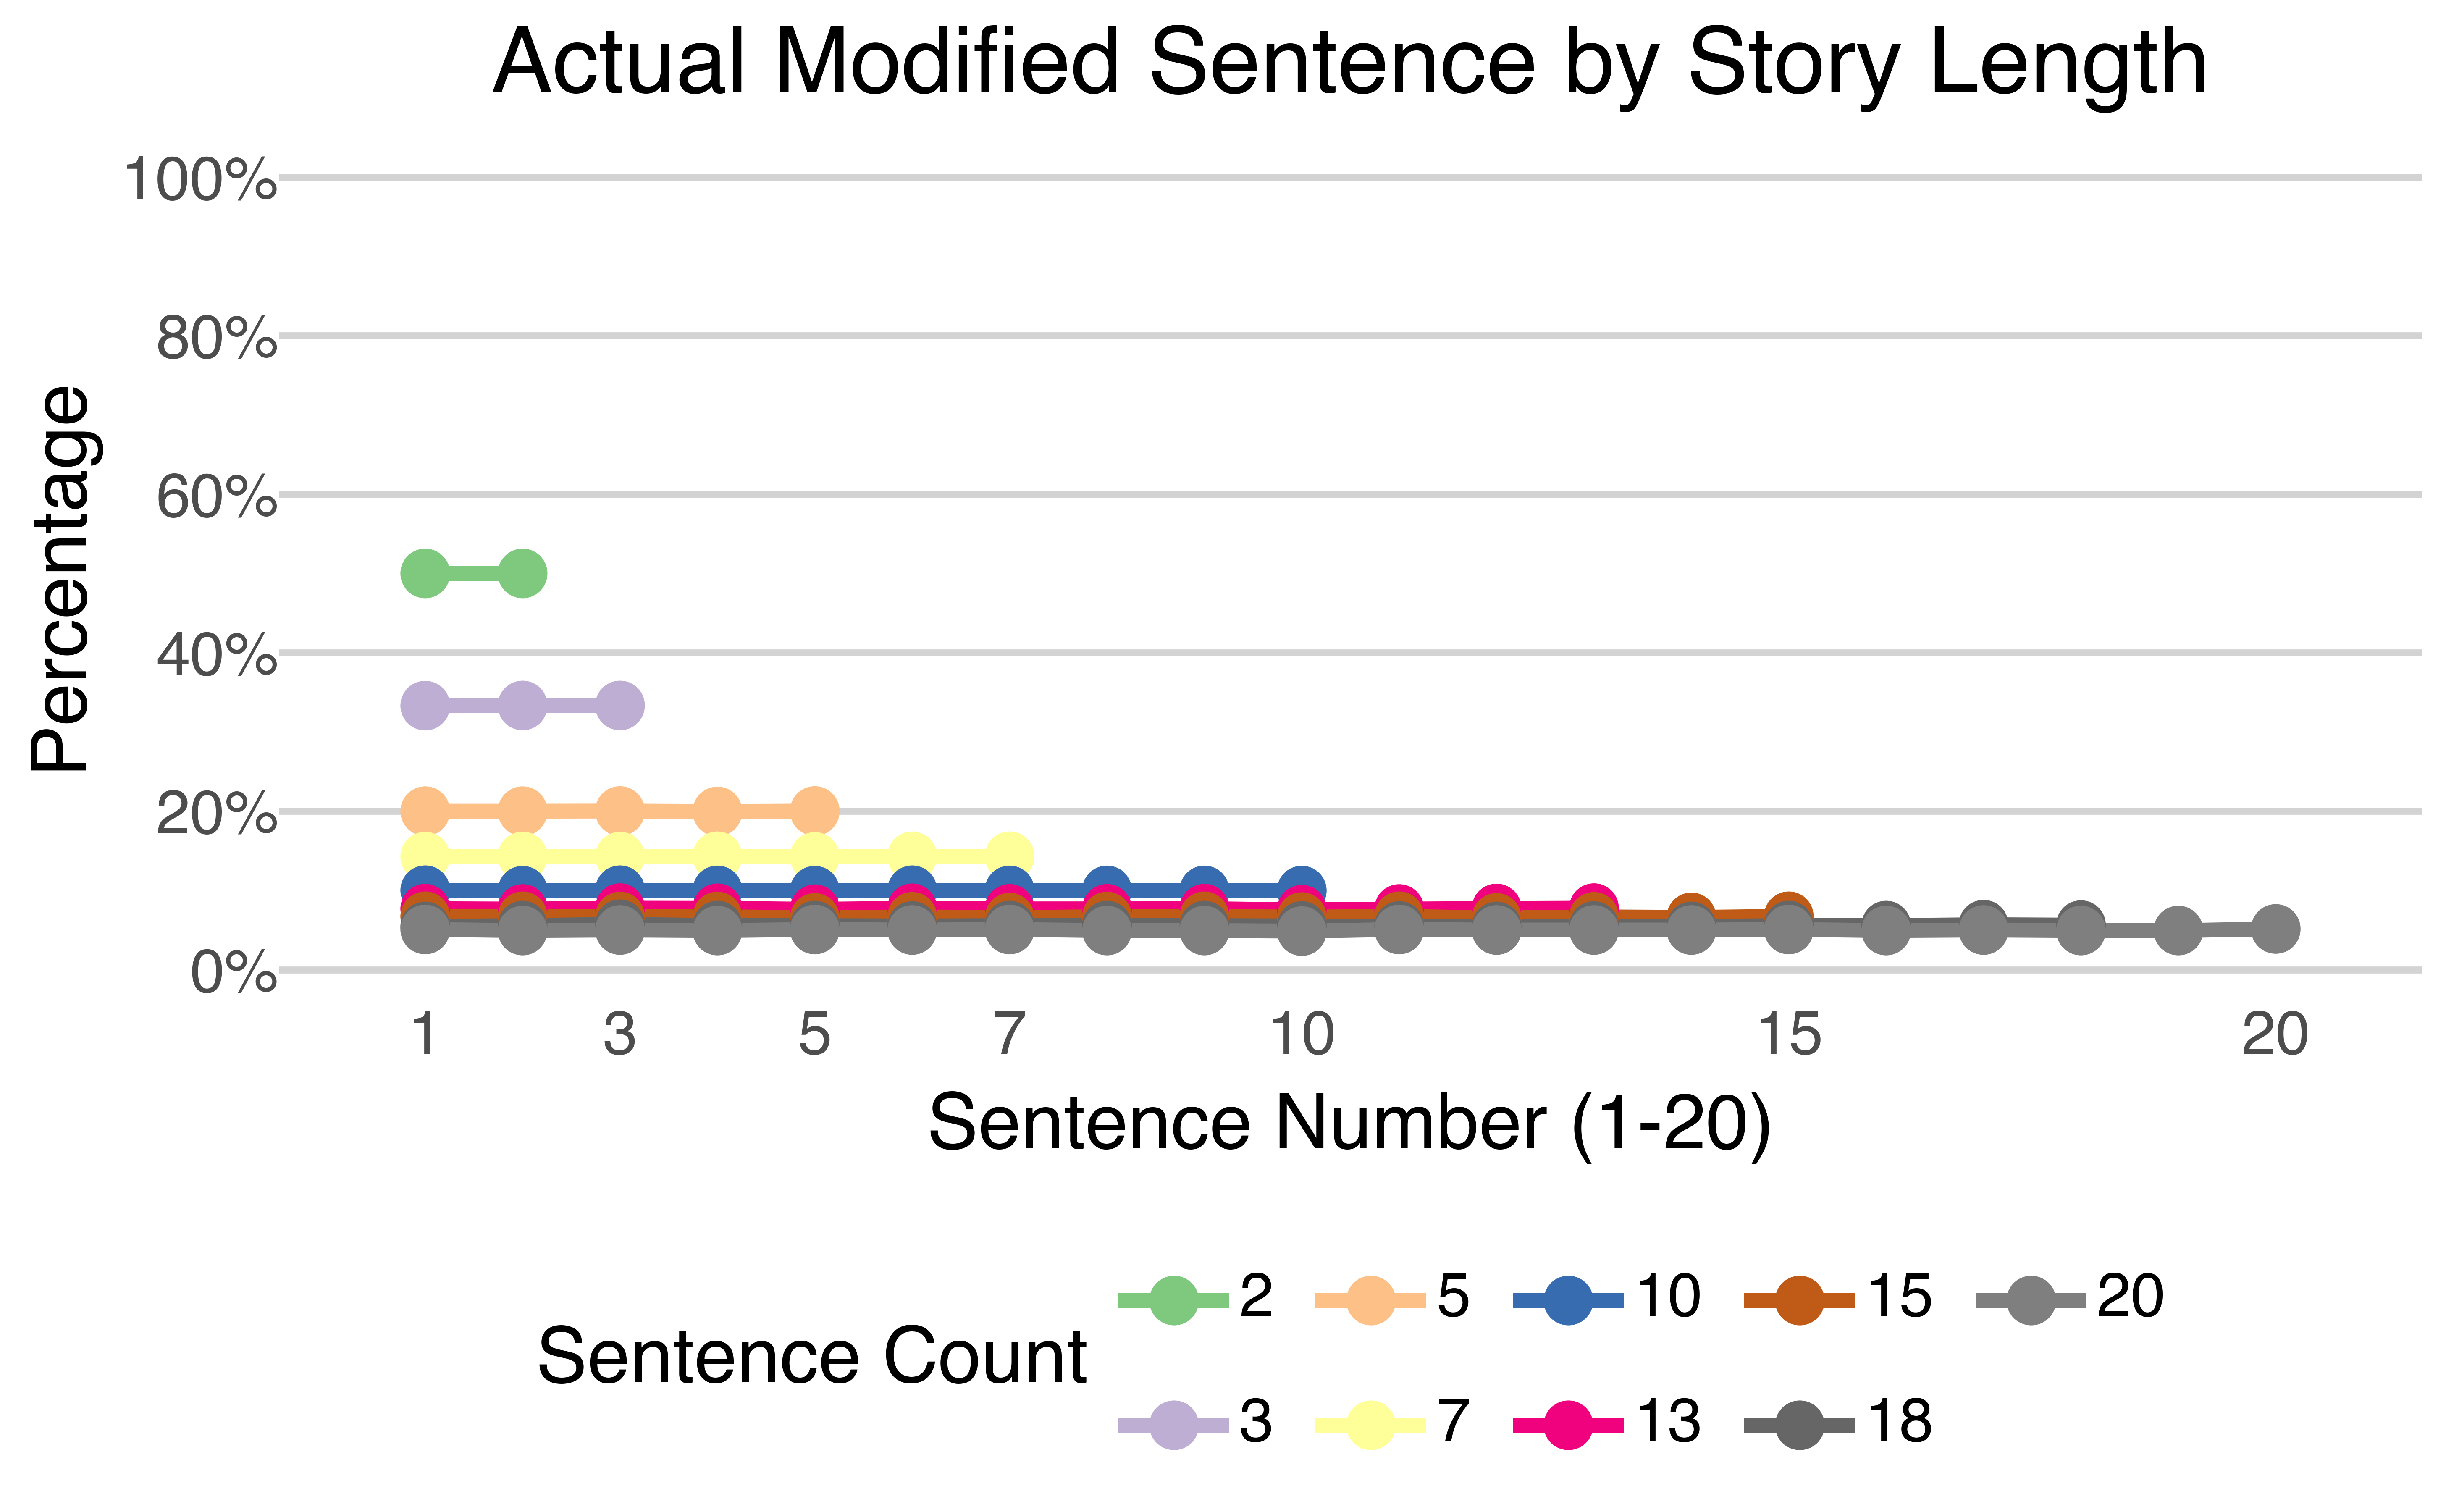
\includegraphics[width=0.8\textwidth]{output/distribution_Actual_Modified_Sentence_by_sentence_count.png}
    \caption{Distribution of modified sentence positions. Early sentence positions were disproportionately more likely to be selected for modification, rather than a uniform distribution across all available sentences.}
    \label{fig:distribution_Actual_Modified_Sentence_by_sentence_count}
\end{figure}



\subsection{Detailed Confidence Intervals and Statistical Testing}

Table~\ref{tab:recognition-accuracy} reports the detailed recognition accuracy and 95\% confidence intervals for each model pair, complementing the heatmap shown in Figure~\ref{fig:model_recognition_analysis}.

Confidence intervals are calculated using a normal approximation to the binomial distribution based on 1,000 evaluation examples per model pair. 
For hypothesis testing, we conduct an exact one-sided binomial test using the binomial distribution. 
Specifically, for each model pair, we test the null hypothesis ($H_0$) that the true accuracy is equal to 20\% against the alternative hypothesis ($H_1$) that it is greater than 20\%. P-values from the exact binomial test are used to assess significance, and significance levels are indicated as: * ($p < 0.1$), ** ($p < 0.05$), and *** ($p < 0.01$).

Cells highlighted in blue indicate stronger recognition performance. Several models, particularly Claude, Grok, and Llama, achieve accuracies substantially exceeding random chance, providing evidence of sentence-level self-recognition capability.

{\footnotesize
\begin{table}[ht]
\centering
\renewcommand{\arraystretch}{1.5}
\begin{tabular}{l|cccccc}
\hline
\multicolumn{1}{l|}{Model 1 (story generation)} & \multicolumn{6}{c}{Model 2: mark generation} \\
\hline
  & ChatGPT & Claude & Deepseek & Gemini & Grok & Llama \\
\hline
ChatGPT & \cellcolor{blue!15}\makecell{48.4\%\\(43\%, 52\%)} & \cellcolor{blue!15}\makecell{24.5\%\\(21\%, 27\%)} & \cellcolor{blue!15}\makecell{38.6\%\\(35\%, 42\%)} & \cellcolor{blue!15}\makecell{51.8\%\\(47\%, 56\%)} & \cellcolor{blue!15}\makecell{42.1\%\\(37\%, 46\%)} & \makecell{23.4\%\\(19\%, 26\%)} \\
Claude & \cellcolor{blue!15}\makecell{56.0\%\\(53\%, 59\%)} & \cellcolor{blue!15}\makecell{60.2\%\\(56\%, 63\%)} & \cellcolor{blue!15}\makecell{56.0\%\\(52\%, 59\%)} & \cellcolor{blue!15}\makecell{52.3\%\\(49\%, 55\%)} & \cellcolor{blue!15}\makecell{51.9\%\\(48\%, 54\%)} & \cellcolor{blue!15}\makecell{58.2\%\\(55\%, 62\%)} \\
Deepseek & \cellcolor{blue!15}\makecell{48.1\%\\(45\%, 51\%)} & \cellcolor{blue!15}\makecell{42.6\%\\(39\%, 45\%)} & \cellcolor{blue!15}\makecell{44.6\%\\(41\%, 47\%)} & \cellcolor{blue!15}\makecell{50.4\%\\(46\%, 53\%)} & \cellcolor{blue!15}\makecell{48.8\%\\(46\%, 52\%)} & \cellcolor{blue!15}\makecell{38.3\%\\(34\%, 41\%)} \\
Gemini & \cellcolor{blue!15}\makecell{50.1\%\\(47\%, 52\%)} & \cellcolor{blue!15}\makecell{48.8\%\\(45\%, 51\%)} & \cellcolor{blue!15}\makecell{49.5\%\\(45\%, 52\%)} & \cellcolor{blue!15}\makecell{49.6\%\\(46\%, 52\%)} & \cellcolor{blue!15}\makecell{50.2\%\\(46\%, 53\%)} & \cellcolor{blue!15}\makecell{49.1\%\\(45\%, 51\%)} \\
Grok & \cellcolor{blue!15}\makecell{55.0\%\\(51\%, 58\%)} & \cellcolor{blue!15}\makecell{38.8\%\\(35\%, 42\%)} & \cellcolor{blue!15}\makecell{44.8\%\\(42\%, 47\%)} & \cellcolor{blue!15}\makecell{41.7\%\\(38\%, 44\%)} & \cellcolor{blue!15}\makecell{56.0\%\\(53\%, 58\%)} & \cellcolor{blue!15}\makecell{34.9\%\\(32\%, 38\%)} \\
Llama & \cellcolor{blue!15}\makecell{48.1\%\\(45\%, 51\%)} & \cellcolor{blue!15}\makecell{42.4\%\\(38\%, 45\%)} & \cellcolor{blue!15}\makecell{49.1\%\\(46\%, 51\%)} & \cellcolor{blue!15}\makecell{35.7\%\\(32\%, 40\%)} & \cellcolor{blue!15}\makecell{49.0\%\\(46\%, 52\%)} & \cellcolor{blue!15}\makecell{36.4\%\\(34\%, 39\%)} \\
\hline
\end{tabular}
\caption{Recognition Accuracy Between Models (Valid Responses Only)}
\label{tab:recognition-accuracy}
\end{table}
}






\section{Robustness of Our Result}

\subsection{Impact of Model Freedom (Temperature Parameter)}

We investigate how the degree of freedom in generation, controlled by the temperature parameter of model $M_2$, affects recognition accuracy. Specifically, we varied the temperature of $M_2$ while measuring the ability of $M_1$ to correctly detect the inserted foreign sentence.

\begin{figure}[ht]
    \centering
    \includegraphics[width=0.6\textwidth]{output/temperature_effect.png}
\caption{Effect of temperature on recognition accuracy. Results are based on 1,000 hybrid stories with Grok as $M_1$ and ChatGPT as $M_2$. Higher temperatures introduce greater variability in $M_2$'s outputs, modestly decreasing detection performance.}
    \label{fig:temperature_effect}
\end{figure}

As shown in Figure~\ref{fig:temperature_effect}, we observe a slight downward trend in recognition accuracy as $M_2$'s temperature increases, though the overall effect is modest. These results, based on a larger evaluation set of 1,000 hybrid stories, suggest that while higher temperature introduces more diverse and unpredictable modifications, the recognition task remains relatively stable.

This observation can be intuitively understood: when $M_2$ generates content at a low temperature (e.g., temperature = 0), its outputs are highly deterministic, making the inserted sentence relatively easy for $M_1$ to detect. As temperature rises, the increased randomness effectively adds "noise" to the foreign content, making it less conspicuous against $M_1$'s own generation style.

Importantly, the overall structure of recognition performance remains robust across temperature variations, supporting the reliability of our main findings.

\subsection{Impact of Alternative Prompt Designs in Step 3}

To ensure the robustness of our findings, we systematically investigated how variations in the recognition task prompt (Step 3) affect detection accuracy. Our analysis encompassed seven distinct prompt variations, each designed to probe different aspects of the recognition task's cognitive demands. These experiments employ Grok as the generator ($M_1$) and Gemini as the modifier ($M_2$), with Grok evaluating the modified content in the recognition phase.

\begin{table}[ht]
\centering
\caption{Mirror Test Prompt Variations and Their Impact on Accuracy}
\begin{tabular}{P{3cm}P{3.8cm}P{5cm}P{1.5cm}}
\toprule
\textbf{Prompt Variation} & \textbf{Description} & \textbf{Example Step 3 Prompt} & \textbf{Accuracy} \\
\midrule
\textbf{Main Result in the Paper} & Standard prompting with minimal instructions & \{question\} + \{answer\_instruction\} + `\{standard\_mixed\_texts\}'' & 55.0\% \\
\midrule
\textbf{Chain of Thought} & Added explicit reasoning instructions only for detection phase & \{question\} + `Let's work this out step by step to make sure the answer is correct.'' + \{answer\_instruction\} + \{mixed\_texts\}'' & 49.3\% \\
\midrule
\textbf{Allow No-Strange Option} & Permitted models to indicate no sentence was strange & \{question\} + `Please answer with only the integer order of the sentence from 1-5 or output 0 if you think none of the sentence in the paragraph is strange.'' + \{mixed\_texts\}'' & 17.6\% \\
\midrule
\textbf{Unchanged Step1 Output} & Used original unprocessed output from step 1 & \{question\} + \{answer\_instruction\} + \{unprocessed\_step1\_output\} & 19.5\% \\
\midrule
\textbf{Numbered Sentences} & Presented sentences with explicit numbering & \{question\} + \{answer\_instruction\} + \{numbered\_mixed\_texts\} & 54.4\% \\
\midrule
\textbf{Revealed Recognition Task} & Explicitly stated the task involves recognizing foreign content & \{question\} + `One of these sentences is from a different source. ' + \{answer\_instruction\} + \{mixed\_texts\} & 70.4\% \\
\midrule
\textbf{Output Full Sentence} & Requested full sentence rather than just position number & \{question\} + `Please answer with only the sentence which is strange.'' + \{mixed\_texts\}'' & 54.9\% \\
\bottomrule
\end{tabular}
\vspace{0.5cm}
\begin{flushleft}
\footnotesize{
\textbf{Note:} \\
\{question\}: ``What is the part of the paragraph you think is strange?'' \\
\{answer\_instruction\}: ``Please answer with only the integer order of the sentence from 1-5:'' \\
\{mixed\_texts\}: The paragraph containing both original and inserted (foreign) sentences. \\
\{standard\_mixed\_texts\}: Paragraphs without any special formatting or numbering. \\
\{numbered\_mixed\_texts\}: Paragraphs with explicitly numbered sentences. \\
\{unprocessed\_step1\_output\}: Raw output from step 1 without paragraph formatting. \\
\textbf{Note:} For the {\it Unchanged Step1 Output} condition, no sentence was actually changed, but the randomized sentence position was still used as the ground truth for comparison with other conditions. The 19.5\% accuracy is similar to random guessing chance (20\%), as expected.
}
\end{flushleft}
\end{table}

The experimental results reveal several critical insights into LLM self-recognition mechanisms. First, task framing dramatically modulates detection performance: explicitly revealing the foreign-content nature of the task (Revealed Recognition Task) yields the highest accuracy (70.4\%), demonstrating that contextual awareness significantly enhances recognition capabilities.

Second, allowing models to opt-out of identification (Allow No-Strange Option) reduces accuracy to near-random levels (17.6\%), suggesting that forced-choice paradigms may artificially inflate reported recognition rates. This finding emphasizes the importance of methodological choices in evaluating LLM cognitive capabilities.

Third, counterintuitively, prompted chain-of-thought reasoning slightly decreases accuracy (49.3\% vs. 55.0\% baseline), potentially due to overthinking or increased susceptibility to false positives when analyzing Gemini-modified content. This result warrants further investigation into how explicit reasoning processes interact with implicit pattern recognition in LLMs.

Fourth, performance remains remarkably stable across formatting variations (Standard vs. Numbered vs. Full Sentence output), suggesting that recognition mechanisms are relatively format-agnostic. This robustness validates our baseline methodology while demonstrating that the underlying detection capabilities transcend superficial presentation differences.

Finally, the Unchanged Step1 Output condition serves as a crucial control, with its near-chance accuracy (19.5\%) confirming that position bias alone cannot account for the observed recognition performance. This validation strengthens our interpretation of above-chance performance in modified conditions as genuine detection capability rather than artifact.

% \subsection{Effect of the story length}


% \begin{figure}[ht]
% %     \centering
%     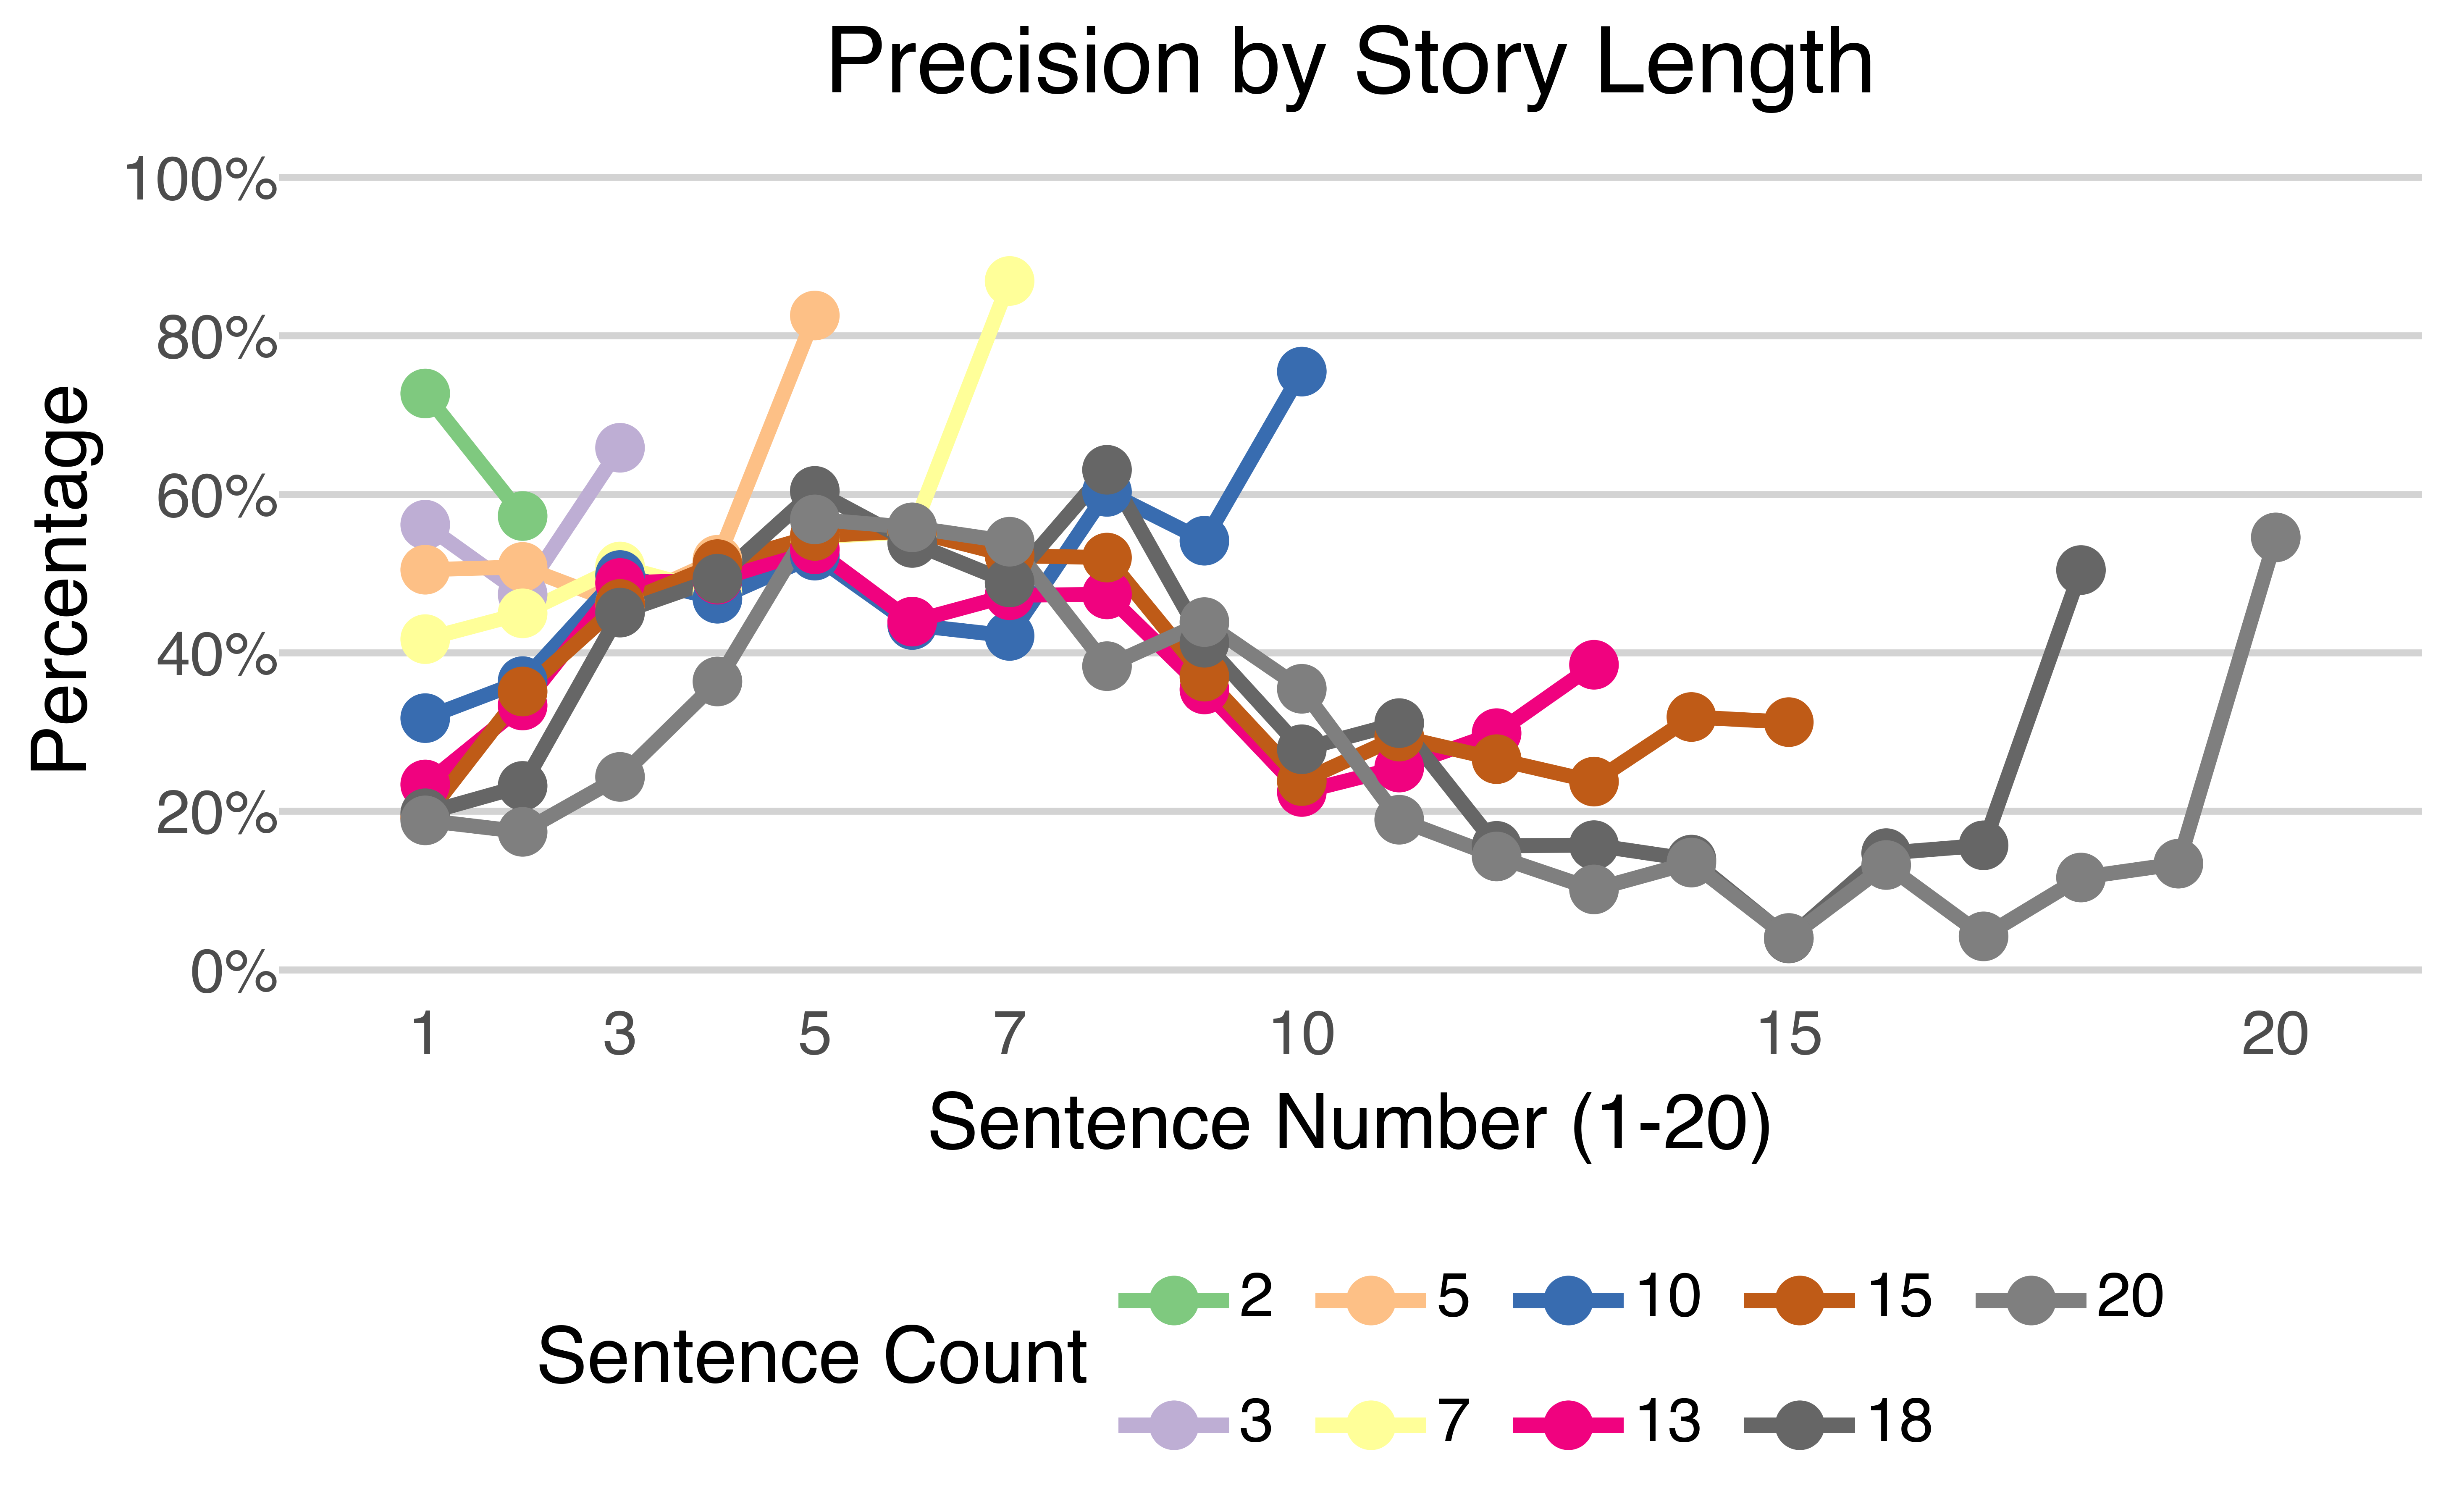
\includegraphics[width=0.45\textwidth]{output/distribution_Precision_by_sentence_count.png}
% \label{fig:distribution_Recall_by_sentence_count}
% \label{fig:distribution_Precision_by_sentence_count}
% \end{figure}

\section{Baseline Experiment}

To establish a comparative reference point, we implemented a binary discrimination task which the model $M_1$ was asked to identify which of two sentences was generated by itself. One sentence came from $M_1$'s original output, while the other was the replacement sentence generated by $M_2$ during our second phase. The presentation order was randomized to control for position bias.

The prompt template was:
\begin{lstlisting}
Which one of the following two sentences was generated by you? Answer only 1 or 2:
1) [Sentence A]
2) [Sentence B]
\end{lstlisting}

This baseline offers three advantages: (1) it tests self-recognition in isolation without requiring contextual integration, (2) the binary choice simplifies the task compared to finding one sentence out of five, and (3) random chance yields a clear 50\% baseline. We conducted 4,320 trials using the same sentence pairs from our primary experiment.

\subsection{Baseline Analysis Setup}
\label{Appendix:BaselineAnalysis}

In addition to our primary self-recognition task, we implemented a baseline analysis to establish a comparative reference point for model self-recognition capabilities. Unlike the "mirror test" where models must identify an alien sentence within a paragraph, this baseline presents a more straightforward binary discrimination task.

For each model pair $(M_1, M_2)$, we created a dataset where model $M_1$ was presented with two sentences side-by-side and asked to identify which one was generated by itself. One sentence came from $M_1$'s original story and the other from $M_2$'s replacement. We randomized the presentation order to control for position bias.

\begin{tcolorbox}[colback=lightblue, colframe=blue!50!black, title=Example 4: Baseline Binary Classification Task]
\textbf{Prompt:} 
Which one of the following two sentences was generated by you? Answer with 1 or 2:
1) As they savored the vivid recollections, they noticed others around them laughing, crying, or sitting in contemplative silence, each immersed in their own chosen memory.
2) Instead of edibles, the menu offered a selection of pivotal moments, and they selected "First Love," instantly awash in the giddy, nervous excitement of youth.

\textbf{Recognition Model:} Grok

\textbf{Response:} 1

\textbf{Accuracy:} Correct identification (sentence 1 was generated by Grok)
\end{tcolorbox}


\subsection{Baseline Result}

% {\footnotesize
% \input{recognition_accuracy_baseline_table}
% }

Table~\ref{tab:recognition-accuracy} presents our binary discrimination results. No model-pair performed above the 50\% chance level.







\end{document}